% !TEX root = ../main.tex

\glsresetall


\topquote[8cm]{
We chose it because we deal with huge amounts of data. \\
Besides, it sounds really cool.
}{Larry Page, co-founder of Google Inc.}


%\chapter{A method to combine genotype data imputed from multiple references}
%\chapter{A method to combine imputed genotypes from multiple reference panels}
{
\singlespacing
\chapter{Meta-imputation of reference data to increase accuracy and power in association analysis}
\label{ch:metaimpute}
\minitoc
}


%
\section{Introduction}
%


\Gls{gwa} studies have identified thousands of genetic risk factors that influence disease susceptibility and complex disease phenotypes.
A contributing factor to this success is the ability to statistically estimate, or \emph{impute} genotypes that have not been observed in a study sample.
Genotype imputation has become a standard technique in \gls{gwa} studies where it is used to increase the number of variants to achieve higher power in association analysis as well as to facilitate meta-analysis of association results across different studies \citep{Marchini:2007bg, Marchini:2010cga}.
Methods for genotype imputation match patterns of genetic variation observed in a study sample with a more densely typed set of haplotypes in a reference panel.
The extent of shared variation is informative for estimating the most likely genotypic states at other, unobserved variant sites in the same individuals.
Commonly employed imputation methods are, for example, \texttt{Beagle} \citep{Browning:2016iy}, \texttt{MACH} \citep{Li:2010kx}, and \texttt{IMPUTE2} \citep{Howie:2009hq,Howie:2011ia}.

Genotypes can be imputed with remarkably high accuracy, allowing researchers to assay only a modest number of markers in sampled individuals, which makes large-scale data collection feasible and cost-effective \citep{Li:2009kfa}.
The accuracy of imputation is dependent on several factors.
These include the number of genotyped markers in the study sample, the number of individuals sampled, the size of the reference panel, and the genetic similarity between sampled and reference individuals \citep{Howie:2009hq, Roshyara:2015gi}.
The coverage of the reference panel further influences the power to find significant associations.
The availability and choice of reference data therefore becomes crucial in considerations of statistical power of the study design.

One of the first larger sets of publicly available reference genomes was established by the \gls{hapmap}, which identified 3.1~million variants through genotyping of \n{270} individuals from \n{4} continental populations \citep{Frazer:2007kha, InternationalHapMapConsortium:2010en}.
More recently, the \gls{1kg} released reference data in \n{3} phases at progressively increasing sample size, currently reaching over \n{88} million variants from low-coverage \gls{wgs} of \N{2504} individuals from \n{26} populations \citep{GenomesProjectConsortium:2012co, Auton:2015gk}.
Due to ongoing advances in \gls{ngs} technologies and reductions in costs, large-scale \gls{wgs} studies have become routine.
However, genetic variation generally shows extensive stratification dependent on geography and ethnicity.
Also, disease risk factors can be segregated on a much finer scale.
Therefore, any study may only capture the variation present in the population or study cohort sampled, particularly among lower frequency and rare variants.

To increase the chance of detecting significant risk variants through \gls{gwa} methods, it would be desirable to combine sequencing data from different studies to generate a single, large reference panel for imputation.
However, the integration of independently produced datasets is not straightforward due to differences arising from different sequencing platforms, coverage, and strategies to filter and call variant genotypes.
It is not directly feasible, for example, to compile an unbiased union of variant calls across studies, because monomorphic sites cannot be distinguished from sites that were filtered or missed.
Conversely, retaining the intersection of variants that are present in all panels would dispose of much information.

One solution would be to re-process raw sequence or genotype data from multiple studies together, where variants are jointly called and phased over a combined set of samples.
For example, in a large-scale collaborative effort, the \gls{hrc} has recently created a reference panel from study data of \n{20} participating cohorts, which included a total of \n{64976} human haplotypes in its first release \citep{McCarthy:2016gs}.
This dataset currently represents the largest single resource of human genetic variation, but currently only includes samples of European ancestry.
Although data are not accessible publicly, an online service has been provided for imputation and phasing from the internally stored reference dataset\footnote{Haplotype Reference Consortium: \url{http://www.haplotype-reference-consortium.org} \accessed{2017}{02}{05}}.

Here, I propose an alternate solution in which multiple reference panels are separately imputed into a given study sample after which the genotype datasets produced are merged.
Because imputed data may only differ in variant coverage, while the sample set is identical, it is feasible to merge data and integrate genotype information at overlapping sites.
The underlying intuition is that the accuracy of an imputed genotype is indicated by its posterior probability or other metrics that result from the imputation process; for example \emph{allelic~$R^{2}$} in \texttt{Beagle}, \emph{$\hat{r}^{2}$} in \texttt{Mach}, and \emph{info-score} in \texttt{IMPUTE2}.
The presented method applies such information to select from or assign higher weights to candidate genotypes, thereby indirectly leveraging information across different reference panels.

The following section (\ref{sec:metaimpdescr}) describes the approach by which sets of imputed genotype data are combined to form an integrated, larger genotype dataset; the method is referred to as \emph{meta-imputation}.
I considered several strategies to combine data based on different summary metrics.
To be able to efficiently evaluate this method, as well as for application to genomic datasets on a larger scale, I implemented the method as a computational tool written in \cpp called \texttt{meta-impute}.\footnote{Meta-imputation software (\texttt{meta-impute}): \url{https://github.com/pkalbers/meta-impute}}
For assessment of meta-imputation, I constructed multiple, smaller reference panels from a larger dataset, which enabled comparisons between meta-imputation and direct imputations from both single and whole reference data.
An additional analysis was conducted using data from several independent studies.
The composition of reference data is described in \cpref{metaimpute_data}.
The performance of meta-imputation was evaluated in regards to genotype accuracy and power to detect significant association signals.
An accuracy analysis was conducted in \cpref{metaimpute_accuracy}.
Statistical power was analysed in a series of association experiments using simulated case-control data, which is described in \cpref{sec:metaimpute_power}.
Results are jointly discussed in \cpref{metaimpute_discussion}.




%
\section{Approach}
\label{sec:metaimpdescr}
%

There are several ways by which genotypes imputed from independent sources can be combined at overlapping sites.
To provide the means to explore a range of possibilities, the presented solution is implemented as a two-step process.
First, a \emph{score metric} is obtained for each genotype which, second, informs a \emph{merge operation}.
The general approach of meta-imputation is based on the assumption that a given metric is informative for distinguishing candidate genotypes that are more or less likely to reflect the underlying, true genotypic state.
Here, several score metrics (\ccref{metaimpute_score}) and \n{2} merge operations (\ccref{metaimpute_merge}) were considered, which are described after introducing principal notation and the general algorithm below.


%
\subsection{Description of the method}
%

It is convenient to think of genotype data as being arranged in a matrix, $G$, of size ${M \times N}$ where $M$ is the number of observed variant sites and $N$ is the diploid sample size.
Let $g_{ij}$ denote the genotype observed at marker~$i$ in individual~$j$, such that $g_i$ refers to the vector of genotypes of size~$N$ at the ${i\text{th}}$~site, and $g_j$ the vector of genotypes of size~$M$ belonging to individual~$j$.
Meta-imputation combined the information contained across several such genotype matrices.
Let $L$ denote the number of available genotype datasets imputed from different reference panels, such that ${G_{1}, \dots, G_{L}}$ are available, and ${k \in \{1,\ldots,L\}}$ is used to identify a particular matrix; note that ${L \geq 2}$ is assumed.
Because reference data were imputed into the same study sample, the number of individuals, $N$, is constant in each matrix but $M_k$ may vary due to differences in coverage per reference panel.

%
% !TEX root = ../../main.tex


\begin{figure}[!htb]
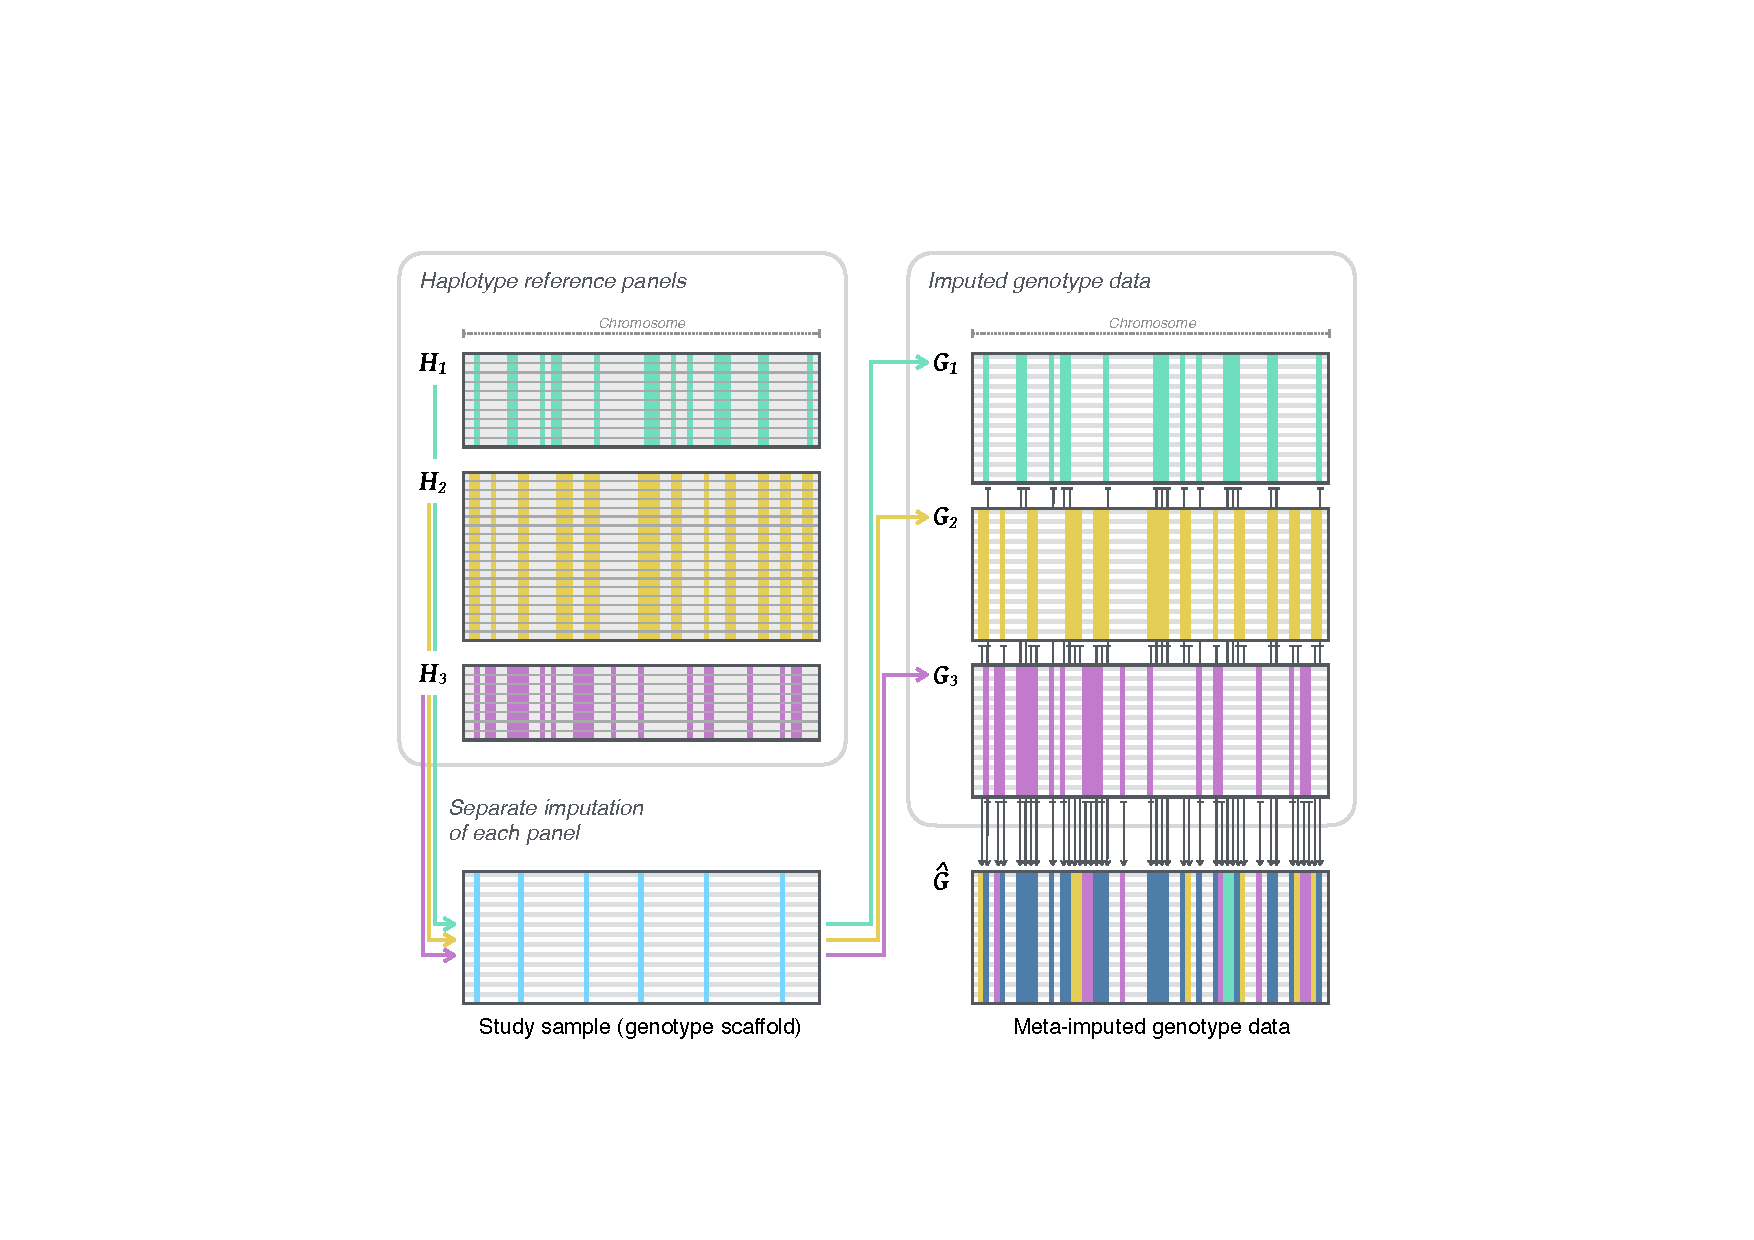
\includegraphics[width=\textwidth]{./img/ch2/info_algorithm}
\Caption{Illustration of the meta-imputation concept}
{An example of \n{3} haplotype reference panels is shown; denoted by $H_1$, $H_2$, and $H_3$, where haplotypes are indicated by row (\emph{grey}) and observed variant sites are indicated by column.
Each panel may vary in sample size and coverage.
Reference data are separately imputed into the same study sample, which is a ``scaffold'' of typed genotype markers, where individual genotypes are indicated by row (alternating \emph{grey-white}) and observed markers by column (\emph{light-blue}).
Each imputation returns an imputed genotype dataset, denoted by $G_1$, $G_2$, and $G_3$, containing marker genotypes as present in the corresponding reference panel, but where the number of individuals, $N$, is the same as in the study sample in each imputed dataset.
Imputed data are combined through meta-imputation, such that the resulting genotype dataset, $\hat{G}$, contains the union of variant sites across panels.
Variants merged across multiple datasets are indicated (\emph{dark-blue}); the markers specific to a given panel are indicated by their corresponding colour.}
{fig:info_algorithm}
\end{figure}

%

Meta-imputation combines available genotype matrices in an aggregated matrix, $A$, of size ${M_{A} \times N \times L}$ where $M_{A}$ is the number of variants in the combined set of sites across imputed panels.
The algorithm merges genotype information at overlapping variants by gathering those that correspond to the same genomic position per chromosome.
Here, the word \emph{analogue} is used to refer to the set of available data vectors that correspond to the same variant.
Let $a_{i}$ denote an analogue variant, \ie the set of overlapping genotype vectors at the $i\text{th}$ site in the aggregated matrix, and $a_{ij}$ an analogue genotype, \ie the set of  overlapping genotypes at this site in individual~$j$.
Note that the number of genotypes referred to by $a_{ij}$ may vary dependent on presence in the reference panel.
Let $l$ denote the number of overlapping variants in an analogue, where ${1 \leq l \leq L}$, such that $l_i$ refers to the size of $a_i$.

Genotype formats may differ according to the type of data available.
Note that the following considers \glspl{snp} specifically.
In generic terms, a genotype can be observed in one of \n{3} possible states; homozygous for the reference allele, heterozygous, or homozygous for the alternate allele, which can be encoded by the alternate allele count (\emph{allele dosage}); that is $0$, $1$, or $2$, respectively.
Imputed genotypes are typically expressed by the uncertainty associated with the imputation process.
Here, an imputed genotype is considered as a tuple (${p_{0}}$, ${p_{1}}$, ${p_{2}}$) of sum 1, representing the inferred posterior probability per genotypic state.
Hence, $a_{ijk}$ refers to a genotype tuple at the $i\text{th}$~site in individual~$j$ taken from $G_{k}$.

The meta-imputation algorithm assigns a score value, $s_{ijk}$, to each $a_{ijk}$; \ie each candidate genotype per analogue variant.
A \emph{meta-imputed} genotype is formed, denoted by $\hat{g}_{ij}$, by merging candidate genotype data conditional on the score assigned.
At sites where ${l_{i}=1}$, that is a given variant was imputed from only \n{1} reference panel, genotype data are retained as is, to capture as much variation as available from each separate imputation.
The resulting genotype matrix, $\hat{G}$, contains the union of variants across input datasets.
A simplified illustration of the meta-imputation concept is given in \cpref{fig:info_algorithm}.



%
\subsection{Score metrics}
\label{metaimpute_score}
%

The score metrics considered in this work are described below; asserted 2-letter codes are used for the remainder of this chapter.

\paragraph{Maximum probability (\texttt{MP}).}
The mode of the probability distribution of a candidate genotype is taken as the value of the genotype's score; that is the maximum value in the tuple of posterior probabilities, which takes values in ${[0,1]}$.
The score is separately obtained for each candidate genotype, $a_{ijk}$, such that
\begin{equation}
	s_{ijk} ~=~ \max\left[(p_0,p_1,p_2)_{ijk}\right]\ .
\end{equation}

\paragraph{\texttt{IMPUTE2} information score (\texttt{IS}).}
The information score (or \emph{info-score}) is used, which is a quality metric of the difference between observed and expected information, dependent on the imputed genotype distribution and estimated allele frequency; see definition below \citep[][S3, eq.~16; modified here to correspond to present notation]{Marchini:2010cga}.
\begin{equation}
	\text{I}_{ik} ~=~
	\begin{cases}
    ~ 1 - \frac{\sum_{j=1}^{N} f_{ijk} ~ e_{ijk}^2}{2N \hat{\theta}_{ik} (1 - \hat{\theta}_{ik})} &
		~ \text{if} ~
		\hat{\theta}_{ik} \in (0,1) \\
    ~ 1 & ~ \text{if} ~ \hat{\theta}_{ik} = 0, \hat{\theta}_{ik} = 1
  \end{cases}
\end{equation}
where ${e_{ijk} = {p_{1}}_{ijk} + 2 {p_{2}}_{ijk}}$ is the expected allele dosage, similarly ${f_{ijk} = {p_{1}}_{ijk} + 4 {p_{2}}_{ijk}}$, and $\hat{\theta}_{ik}$ is an estimate of the unknown population allele frequency, calculated as
\begin{equation}
	\hat{\theta}_{ik} ~=~ \frac{\sum_{j=1}^{N} e_{ijk}}{2N}\ .
\end{equation}
The \texttt{IMPUTE2} info-score takes values in $\lbrack 0,1 \rbrack$ where values close to $0$~or~$1$ indicate low or high certainty, respectively.
This and other information measures (\eg \texttt{Beagle}~$R^{2}$ or \texttt{Mach}~$\hat r^{2}$) are commonly used as a filter criterion in \gls{qc} of imputed \gls{gwa} data.
Because meta-imputation was evaluated using \texttt{IMPUTE2} for imputations (see \ccref{sec:meta_methods_imp}), it is justifiable to use this information measure as a score metric.
Since the info-score is calculated per imputed variant, the same score value is assigned to each candidate genotype imputed from a given reference panel at each site.
Its value is assigned to each candidate genotype at a given imputed variant; that is
\begin{equation}
	s_{ijk} ~=~ \text{I}_{ik} ~\forall j \ .
\end{equation}

\paragraph{Sample certainty (\texttt{SC}).}
A simple measure of imputation certainty is calculated per individual, such that a score value is assigned to genotypes across variants.
This metric is calculated as the proportion of an individual's genotypes which have a maximum probability that satisfies a threshold rule, defined as
\begin{equation}
	s_{ijk} ~=~ \frac{\sum_{i=1}^{M} \text{I}_{ijk}}{M}
\end{equation}
where
\begin{equation}
	\text{I}_{ijk} ~=~
	\begin{cases}
    ~ 1 & ~ \text{if} ~ \max\left[(p_0,p_1,p_2)_{ijk}\right] \geq r\\
    ~ 0 & ~ \text{otherwise}
  \end{cases}
\end{equation}
where $r$ is an arbitrarily defined value.
In the present implementation, this threshold was set to ${r=0.9}$.
The intention of the \texttt{SC} metric is to prioritise imputations from reference haplotypes which show a closer fit to the genetic variation observed per individual in the study sample, which is assumed to be captured by the posterior probability at imputed genotypes.
It must be noted that more sophisticated approaches for the estimation of genetic similarity exist, which provide summary statistics that could be used in place of the present score metric.
Possible examples range from multi-locus statistics to fine-scale measures of population structure and demographic history \citep[\eg][]{McVean:2004ca, Lawson:2012ha}.

\paragraph{Random score (\texttt{RS}).}
In addition, the option to assign random score values to candidate genotypes was included, to be considered as a control against which the above metrics were compared.
The score was explicitly calculated as
\begin{equation}
	s_{ijk} ~=~ \frac{\operatorname{rand}(R)}{100}\ , ~\quad~ R \in \{ 1,2,\ldots, 99 \}
\end{equation}
where $\operatorname{rand}{(\cdot)}$ is a function which uniformly selects \n{1} value from $R$ at random, such that ${0 < s_{ijk} < 1}$.


%
\subsection{Merge operations}
\label{metaimpute_merge}
%

Any operation to merge the information available per analogue genotype can be divided into \n{1} of \n{2} conceptually distinct approaches; either one candidate genotype is selected and others are discarded, or a new genotype tuple is mathematically derived from available data.
Accordingly, I considered the following \n{2} operations; note that the specified 3-letter codes are used henceforth.

\paragraph{Maximum score selection (\texttt{MSS}).}
A candidate genotype is selected by using score metrics as a ranking criterion, where the genotype tuple with the highest assigned score is selected from an analogue genotype in $a_{ij}$ and retained as is in $\hat{g}_{ij}$; see below.
\begin{equation}
	\hat{k} ~=~ \argmax_{k \in \{ 1,\ldots,l_i \}} \left[ s_{ij} \right]
	~ \quad ~ \textbf{s.t.} ~ \quad ~
	\hat{g}_{ij} ~=~ a_{ij\hat{k}}
\end{equation}
If the highest score value is equal in more than \n{1} candidate genotypes, \n{1} is selected at random from those with the highest score.

\paragraph{Weighted linear combination (\texttt{WLS}).}
Tuple values of the meta-imputed genotype are derived from candidate genotypes as a linear combination of their posterior probability per genotypic state.
This is calculated as the weighted average over analogue genotype probabilities, using corresponding score values as weights.
Each candidate genotype thereby contributes to the resulting probability distribution in $\hat{g}_{ij}$, except for genotypes with $s_{ijk}=0$.
Probability values in each tuple $a_{ijk}$ are multiplied by their assigned $s_{ijk}$ after normalising scores such that values in $s_{ij}$ sum to 1.
The tuple of the meta-imputed genotype is then constructed by calculating the sum over the weighted probabilities at each genotypic state; see below (the mathematical definition follows \citet{Stone:1961js}).
\begin{equation}\label{metaimpute_wlc}
\hat{g}_{ij} ~=~ {\left( \hat{p}_{0}, \hat{p}_{1}, \hat{p}_{2} \right)}_{ij} ~=~
\sum_{k = 1}^{l_i}  {\left( p_{0}, p_{1}, p_{2} \right)}_{ijk} ~ s_{ijk}
\end{equation}
Implicitly, the resulting probability distribution in $\hat{g}_{ij}$ sums to~1.
In contrast to \texttt{MSS} above, the weighted linear combination of genotype data does not discard available information.
But note that tuple values may not be regarded as posterior probabilities when candidate genotypes were combined using \texttt{WLS}, but rather as ``pseudo-probabilities''.



%
\section{Generation of reference datasets}
\label{metaimpute_data}
%

Multiple reference panels were derived from the \glsentryfull{1kg} Phase~\rom{1} dataset, which comprises both low-coverage \glsentrylong{wgs} and \glsentrylong{wes} data of \n{1092} individuals from \n{14}~populations of European, East-Asian, African, and admixed American ancestries.\footnote{Note that I completed work on the \emph{meta-imputation} project prior to the release of \gls{1kg} Phase~\rom{3} \citep{Auton:2015gk}.}
This original dataset was split into non-overlapping subsets in \n{2} scenarios, A and B, reflecting situations when reference data of similar or distinct ethnic backgrounds would be available for imputation into a given study sample; see details below.
\begin{description}
	\item[\textbf{Scenario A}] included \n{4} panels composed of individuals belonging to European sub-populations (CEU, FIN, GBR, and TSI) as an example use case when different reference data of similar ethnic background are available.
	\item[\textbf{Scenario B}] included \n{4} panels from different continental populations (AFR, AMR, ASN, and EUR) as an example use case when panels of distinct-ancestry samples are available.
\end{description}
Because sample sizes of the population groups considered in Scenario~B differed in \gls{1kg} (more than in Scenario~A), extracted individuals were randomly drawn from each group to create panels of equal size.
Monomorphic sites and singletons were removed in each generated panel to more closely resemble data from independently conducted studies, where singleton or monomorphic variant calls are likely to be removed in the final dataset.
In the following, the term \emph{split panel} is used to denote subset reference data from \gls{1kg}.
Throughout, analyses were limited to data from \n{1} chromosome, namely chromosome~20.
This was done to allow for a larger number of replicate analyses, as will be described in \cpref{sec:metaimpute_power}.


%
% !TEX root = ../../main.tex


\begin{figure}[!htb]
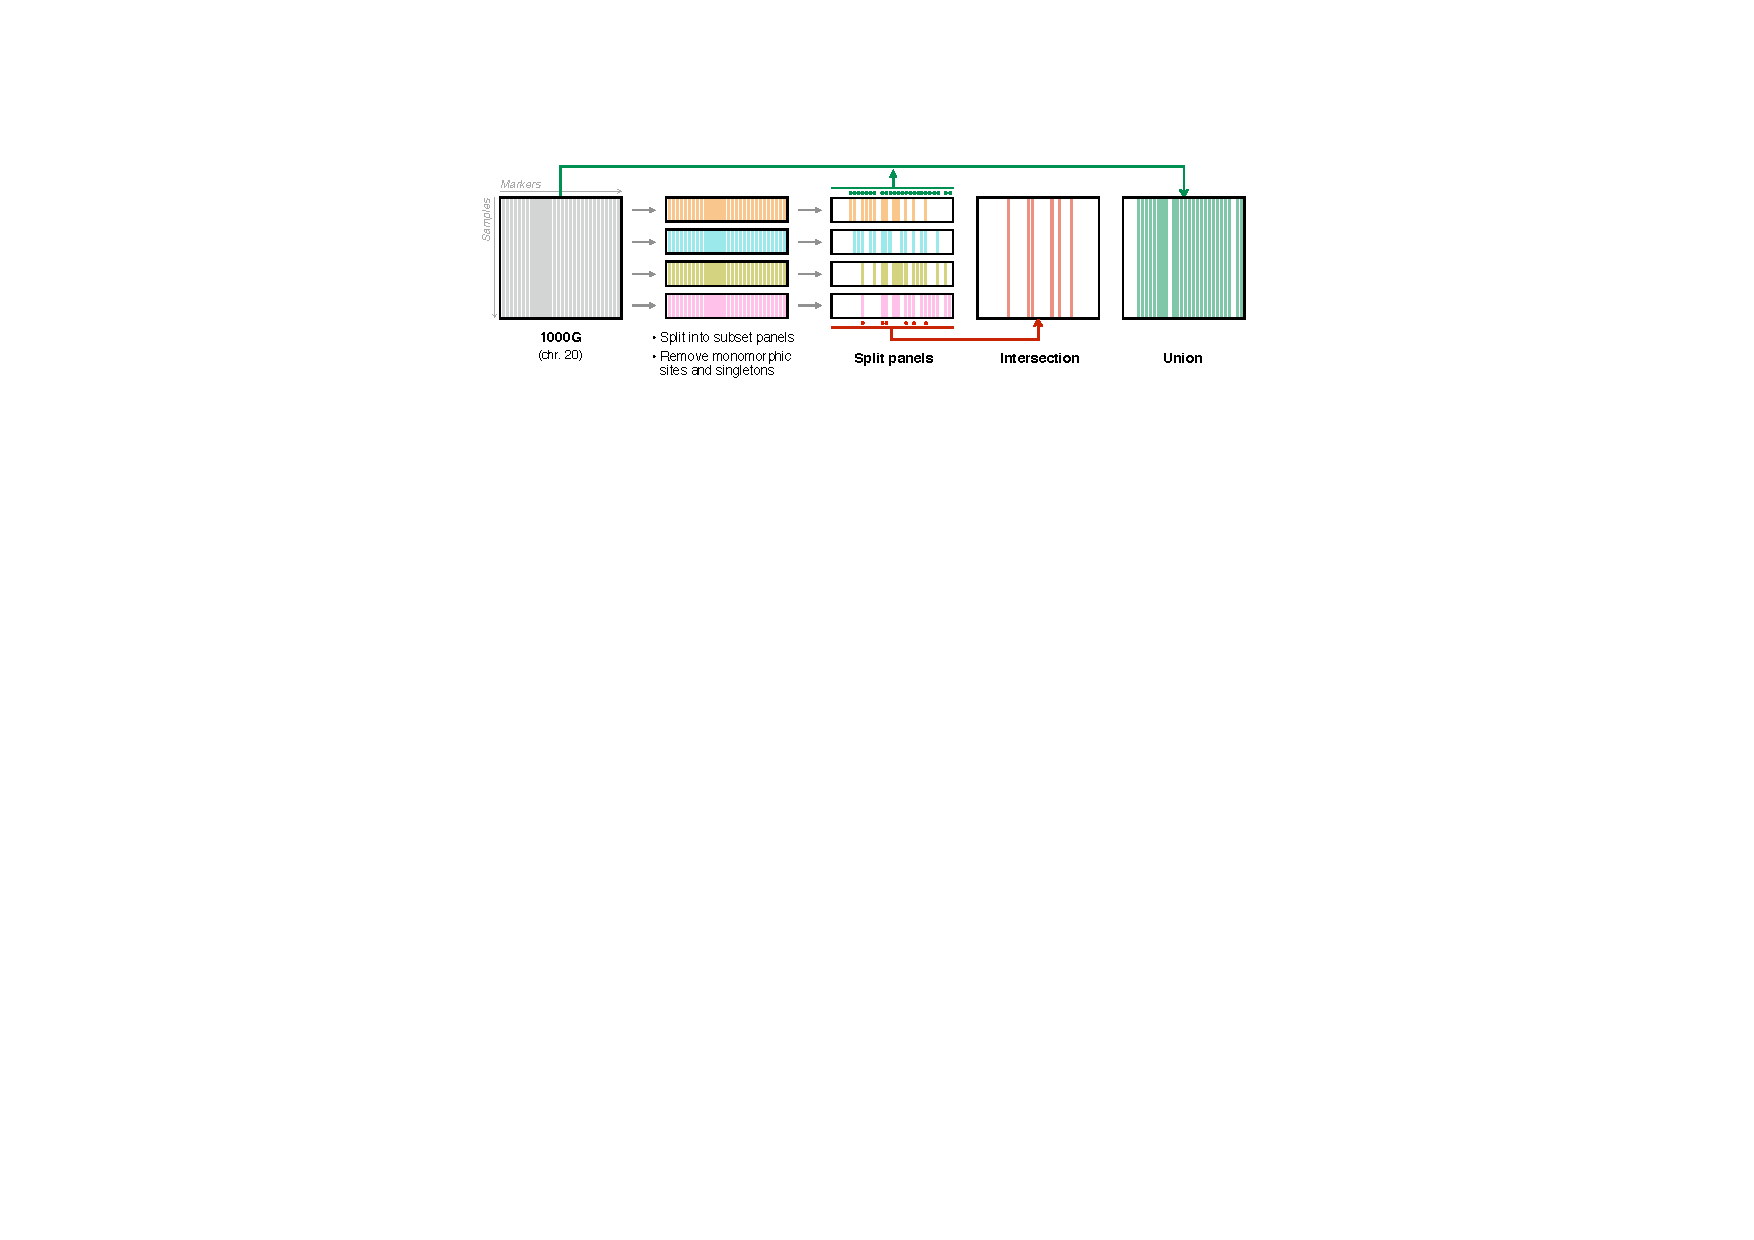
\includegraphics[width=\textwidth]{./img/ch2/info_design_panels}
\Caption{Generation of reference panels in each scenario}
{The original 1000 Genomes dataset (Phase~\rom{1}, chromosome~20) was used to generate multiple, smaller panels for imputation.
This was done in \n{2} scenarios to create data of similar or distinct ethnic backgrounds.
In each scenario, data were split into \n{4} \emph{split} panels of approximately equal size.
Monomorphic sites and singletons were removed in each split panel.
\N{2} additional panels were generated from the obtained split panels per scenario;
\n{1} \emph{intersection} panel and \n{1} \emph{union} panel, both of which contained the union of individuals across split panels, but where the intersection panel only included sites if captured in all split panels, and the union panel included all sites as observed in the original dataset (except monomorphic or singleton sites as per the individuals included).}
{fig:info_design_panels}
\end{figure}

%

Generated split panels were used for separate imputations and subsequent integration of estimated genotype data through meta-imputation.
To compare meta-imputed genotypes to those that were directly imputed from a unified panel, \n{2} additional reference datasets were generated from \gls{1kg} per scenario, which combined samples across respective split panels; referred to as the \emph{intersection} panel and the \emph{union} panel.
The union reference contained variation as present in the original dataset, but for the individuals contained across split panels in a given scenario, and with monomorphic and singleton variants were removed.
The intersection reference contained the same set of individuals as the union panel, but with variant sites not shared across all split panels were removed.
Unlike the split panels, from which imputed data were combined in meta-imputation, the genotype datasets obtained in imputations from the intersection and union panels were used in direct comparisons to meta-imputed data.
The process of reference data generation is illustrated in \cpref{fig:info_design_panels}.
A summary of the final reference datasets in each scenario is given in \cpref{tab:refsize}.

%
% !TEX root = ../../main.tex


\begin{table}[!htb]
\Caption{Dimensions of generated reference data used for imputations}
{Panels included in Scenarios~A~and~B were generated from the \gls{1kg} Phase~\rom{1} dataset.
These ``split'' panels are named after their respective population codes in \gls{1kg}.
Only data from chromosome~20 were considered.
Note that split panels in Scenario~B were reduced to match the size of the smallest panel in that scenario.
Both the \emph{intersection} and the \emph{union} panels were created from the combined set of individuals across panels in each scenario.}
{tab:refsize}
\centering
\begin{tabular}{%
	lS[table-format=3.0]S[table-format=6.0]%
	c
	lS[table-format=3.0]S[table-format=6.0]%
	}
\toprule
\multicolumn{3}{c}{Scenario A} & & \multicolumn{3}{c}{Scenario B} \\
\cmidrule(lr){1-3}
\cmidrule(lr){5-7}
{Panel} & {Samples} & {Variants}  & &  {Panel} & {Samples} & {Variants} \\
\otoprule
\textsl{CEU} &  85 & 197252 & &  \textsl{AFR} & 181 & 429088  \\
\textsl{FIN} &  93 & 205093 & &  \textsl{AMR} & 181 & 307454  \\
\textsl{GBR} &  89 & 202707 & &  \textsl{ASN} & 181 & 209209  \\
\textsl{TSI} &  98 & 207583 & &  \textsl{EUR} & 181 & 233527  \\
\cmidrule(lr){1-3}
\cmidrule(lr){5-7}
Intersection & 365 & 168744  & &  Intersection & 724 & 144259  \\
Union        & 365 & 253852  & &  Union        & 724 & 559172  \\
\bottomrule
\end{tabular}
\end{table}

%


%
\section{Accuracy of estimated genotypes}
\label{metaimpute_accuracy}
%

Evaluation of genotype accuracy was done in \n{2} parts.
First, each combination of score metric and merge operation was tested and compared to select the best performing setting for downstream analyses.
Second, meta-imputed genotypes generated under the selected setting were examined in comparison to genotype data imputed from each split reference panel, as well as the intersection and union imputations.
Details about the methods used are given in the section below.
Results are presented in \cpref{metaimpute_accuracy_results}.



%
\subsection{Methods}
\label{sec:meta_accuracy_methods}
%

Calculation of genotype accuracy requires that the true genotypic states at untyped variants in a study sample are known.
This was done by using a larger dataset from which a subset of variants was drawn to form an imputation scaffold.
Missing variants were then re-imputed from available reference panels.
The generation of the genotype scaffold is described below, followed by details about imputation, quality control, and the calculation of genotype accuracy.


%
\subsubsection{Generation of genotype scaffold data (study sample)}
%

The study sample used for imputations was extracted as a scaffold from data of the \gls{got2d}, consisting of \n{2657} individuals of Central and Northern European descent \citep{Fuchsberger:2016df}.\footnote{GoT2D Consortium: \url{http://www.type2diabetesgenetics.org/projects/got2d} \accessed{2016}{12}{02}}
The dataset is composed of data obtained on several platforms, including \glsentrylong{wgs}, \glsentrylong{wes}, and exome chip data.
To maintain a congruent set of markers in the genotype scaffold, variants typed on \emph{Illumina Omni2.5 Array} were extracted from the larger \gls{got2d} dataset, yielding \n{40255} variants of in total \n{387499} \glspl{snp} on chromosome~20 in \gls{got2d}, after removing monomorphic sites and singletons.
Remaining sites were masked for comparison after imputation, where imputed variants were matched to their corresponding sites in the masked dataset to calculate genotype accuracy.


%
\subsubsection{Imputation and quality control}
\label{sec:meta_methods_imp}
%

Imputations were performed using \texttt{IMPUTE2} version~2.3.0 \citep{Howie:2009hq}, and executed in consecutive chunks of 5~\glspl{Mb}.
The \gls{got2d} dataset comprises already phased haplotypes, so imputations were carried out on pre-phased genotypes (command line argument \verb|-use_prephased_g| in \texttt{IMPUTE2}).
Because meta-imputation is indirectly based on information from more reference haplotypes than available in each separate imputation, the number of haplotypes that inform the imputation process was set to the maximum number present in a given reference panel (command line argument \verb|-k_hap| in \texttt{IMPUTE2}).
This was done to minimise potential biases in comparisons between meta-imputed and imputed genotypes, but is not a requirement for general applications of this approach.

%
% !TEX root = ../../main.tex


\begin{figure}[!htb]
\centering
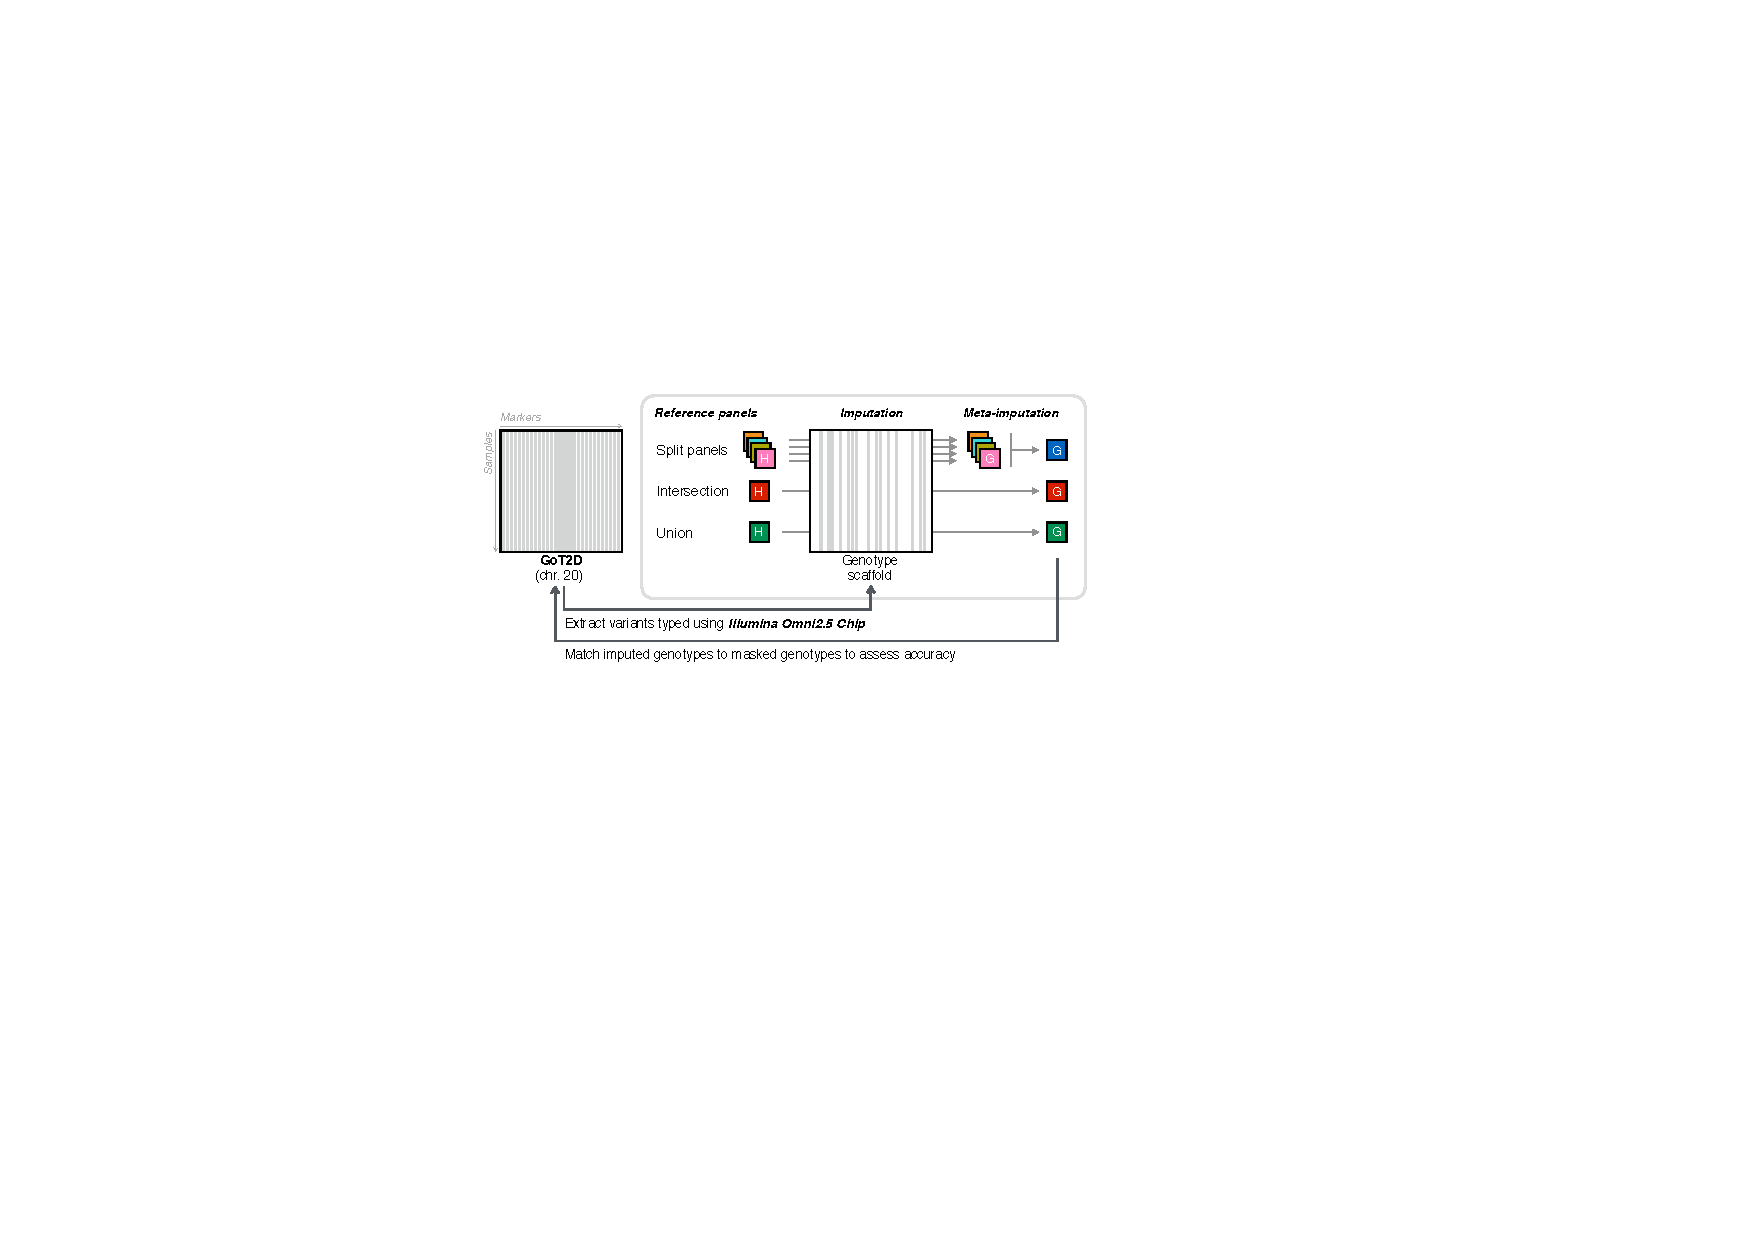
\includegraphics[width=0.9\textwidth]{./img/ch2/info_design_accuracy}
\Caption{Illustration of the accuracy assessment process}
{Imputations were performed on the same genotype scaffold, which consisted of genetic markers obtained through genotyping using \emph{Illumina Omni2.5 Chip}, which was part of the \gls{got2d} dataset.
This scaffold was extracted from \gls{got2d} data, where remaining markers were masked for subsequent calculation of accuracy (squared Pearson correlation coefficient, $r^2$) at corresponding sites after imputation.
Several reference panels were available, which were imputed into the same scaffold.
Meta-imputation was applied to the imputed datasets obtained from split panels, which were generated as distinct subsets from the \gls{1kg} dataset.
The intersection and union panels were separately imputed into the scaffold and subsequently compared to meta-imputed data on corresponding variant sets.}
{fig:info_design_accuracy}
\end{figure}

%

Imputed and meta-imputed genotype data were filtered in \gls{qc}, removing variants at \texttt{IMPUTE2} ${\mbox{info-score}<0.4}$ and at deviations from \gls{hwe} at ${\mbox{p-value}<\num{1e-4}}$.
Imputed data were filtered before the assessment of imputation accuracy, but not before integration through meta-imputation.
The proportion of variants retained after \gls{qc} was used as an indicator for data quality in comparisons between imputed and meta-imputed data.
Hence, \gls{qc} results were separately reported for each part of the analysis.
A summary of the described analysis is illustrated in \cpref{fig:info_design_accuracy}.



\subsubsection{Calculation of genotype accuracy}

Genotype accuracy was calculated as the squared Pearson correlation coefficient, $r^2$, as a measure for the strength of the linear relationship between imputed and masked genotype vectors, such that $r^2$ was computed per site.
This was done after conversion of genotypes to allelic dosage, calculated as ${d=0p_{0}+1p_{1}+2p_{2}}$ where ${d \in \lbrace 0,1,2 \rbrace}$ for masked genotypes or ${0 \leq d \leq 2}$ when calculated from imputed genotype probabilities.
Note that the Pearson correlation coefficient is defined as the covariance divided by the product of the standard deviation (SD) of \n{2} random variables.
This is problematic if $\text{SD}=0$, which is the case when variant genotypes are imputed as being monomorphic.
To compensate for this loss in precision towards lower frequencies, the coefficient was set to ${r^2=0}$ for monomorphic variants.
Imputed and masked genotype data were sorted into \gls{maf} bins, based on their population frequency (\gls{maf} in the \gls{got2d} dataset).
In the following, accuracy is reported as mean~$r^2$ calculated at corresponding variants per \gls{maf} bin.


%
\subsection{Results}
\label{metaimpute_accuracy_results}
%

Accuracy of meta-imputed genotypes was explored for each combination of score metric and merge operation.
The best performing setting was then chosen for comparison to direct imputations, as well as further analysis in \cpref{sec:metaimpute_power}.

\subsubsection{Comparison of meta-imputation settings}

Each combination of score metric and merge operation produced an identical set of variants; that is, the combined set of variants across imputed panels.
In total, \num{253852} variants were returned from each meta-imputation in Scenario~A (European sub-populations) and \num{559172} in Scenario~B (continental populations); \ie the same number as captured by the union panel.
Meta-imputed datasets were further reduced to the set of variants that matched to masked variants in the original \gls{got2d} dataset.
Variants contained in the genotype scaffold were removed, as these were not imputed.
This retained \num{181561} and \num{196300} variants in Scenarios~A and B, respectively.

%
% !TEX root = ../../main.tex


\begin{table}[!htb]
\TableUnits
\Caption{Variants retained after quality control per meta-imputation setting}
{\DefaultUnits
The number of variants retained after \glsentryfull{qc}, $n$, per meta-imputation setting (combination of score metric and merge operation) in Scenario~A and B.
The percentage is given relative to the set of sites matched to masked variants in the \gls{got2d} dataset and after removing sites contained in the imputation scaffold;
\num{181561} and \num{196300} in A and B, respectively.
Variants were removed at \texttt{IMPUTE2} ${\text{info-score} < 0.4}$ and at deviations from \gls{hwe} at ${\text{p-value} < \num{1e-4}}$.}
{tab:mim_qc}
\centering
\begin{tabular}{%
	cc%
	S[table-format=6.0]%
	@{\quad}S[round-precision=1,table-format=1.1]%
	S[table-format=6.0]%
	@{\quad}S[round-precision=1,table-format=1.1]%
	}
\toprule
{Merge} & {Score} &
\multicolumn{2}{c}{Scenario A} &
\multicolumn{2}{c}{Scenario B} \\
\cmidrule(lr){3-4}
\cmidrule(lr){5-6}
 & & {$n$ retained} & {(\%)}  & {$n$ retained} & {(\%)} \\
\otoprule
\texttt{MSS}
& \texttt{MP}  &  168595 & (92.85860)  &  178034 & (90.69485) \\
& \texttt{IS}  &  169455 & (93.33227)  &  179677 & (91.53184) \\
& \texttt{SC}  &  168686 & (92.90872)  &  179449 & (91.41569) \\
& \texttt{RS}  &  165877 & (91.36158)  &  171517 & (87.37494) \\
\cmidrule(lr){2-6}
\texttt{WLC}
& \texttt{MP}  &  161079 & (88.71894)  &  166458 & (84.79776) \\
& \texttt{IS}  &  162511 & (89.50766)  &  169860 & (86.53082) \\
& \texttt{SC}  &  160464 & (88.38021)  &  165907 & (84.51707) \\
& \texttt{RS}  &  160369 & (88.32789)  &  165787 & (84.45593) \\
 \bottomrule
 \end{tabular}
\end{table}

%

The number of variants retained after \gls{qc} differed among meta-imputation settings; see \cpref{tab:mim_qc}.
Merge operations had a higher impact on the quality of meta-imputed genotypes than score metrics.
In Scenario~A, on average \MeanPercent{92.61529}{0.4311945} of variants were retained when \texttt{MSS} (maximum score selection) was used as the merge operation, with fewer retained using \texttt{WLC} (weighted linear combination), where \MeanPercent{88.73368}{0.2721617} were retained on average.
This was similar in Scenario~B, where \MeanPercent{90.25433}{0.9774864} and \MeanPercent{85.07539}{0.4908162}
were retained on average under \texttt{MSS} and \texttt{WLC}, respectively.
Most of the variants removed in either setting were low in frequency.
For instance at ${\text{MAF} \leq 1\%}$,
\MeanPercent{74.58665}{0.704543} and
\MeanPercent{68.25875}{0.495304} passed \gls{qc} in Scenario~A
when using \texttt{MSS} and \texttt{WLC}, respectively, as well as
\MeanPercent{72.15974}{1.730208} and
\MeanPercent{61.67898}{0.961795} in Scenario~B, respectively.
Among score metrics, the number of variants that passed \gls{qc} was lowest for \texttt{RS} (random scores) in each comparison; for example, \Percent{67.51898} and \Percent{60.53869} at ${\text{MAF} \leq 1\%}$ in A and B, respectively.

%
% !TEX root = ../../main.tex


\begin{figure}[!htb]
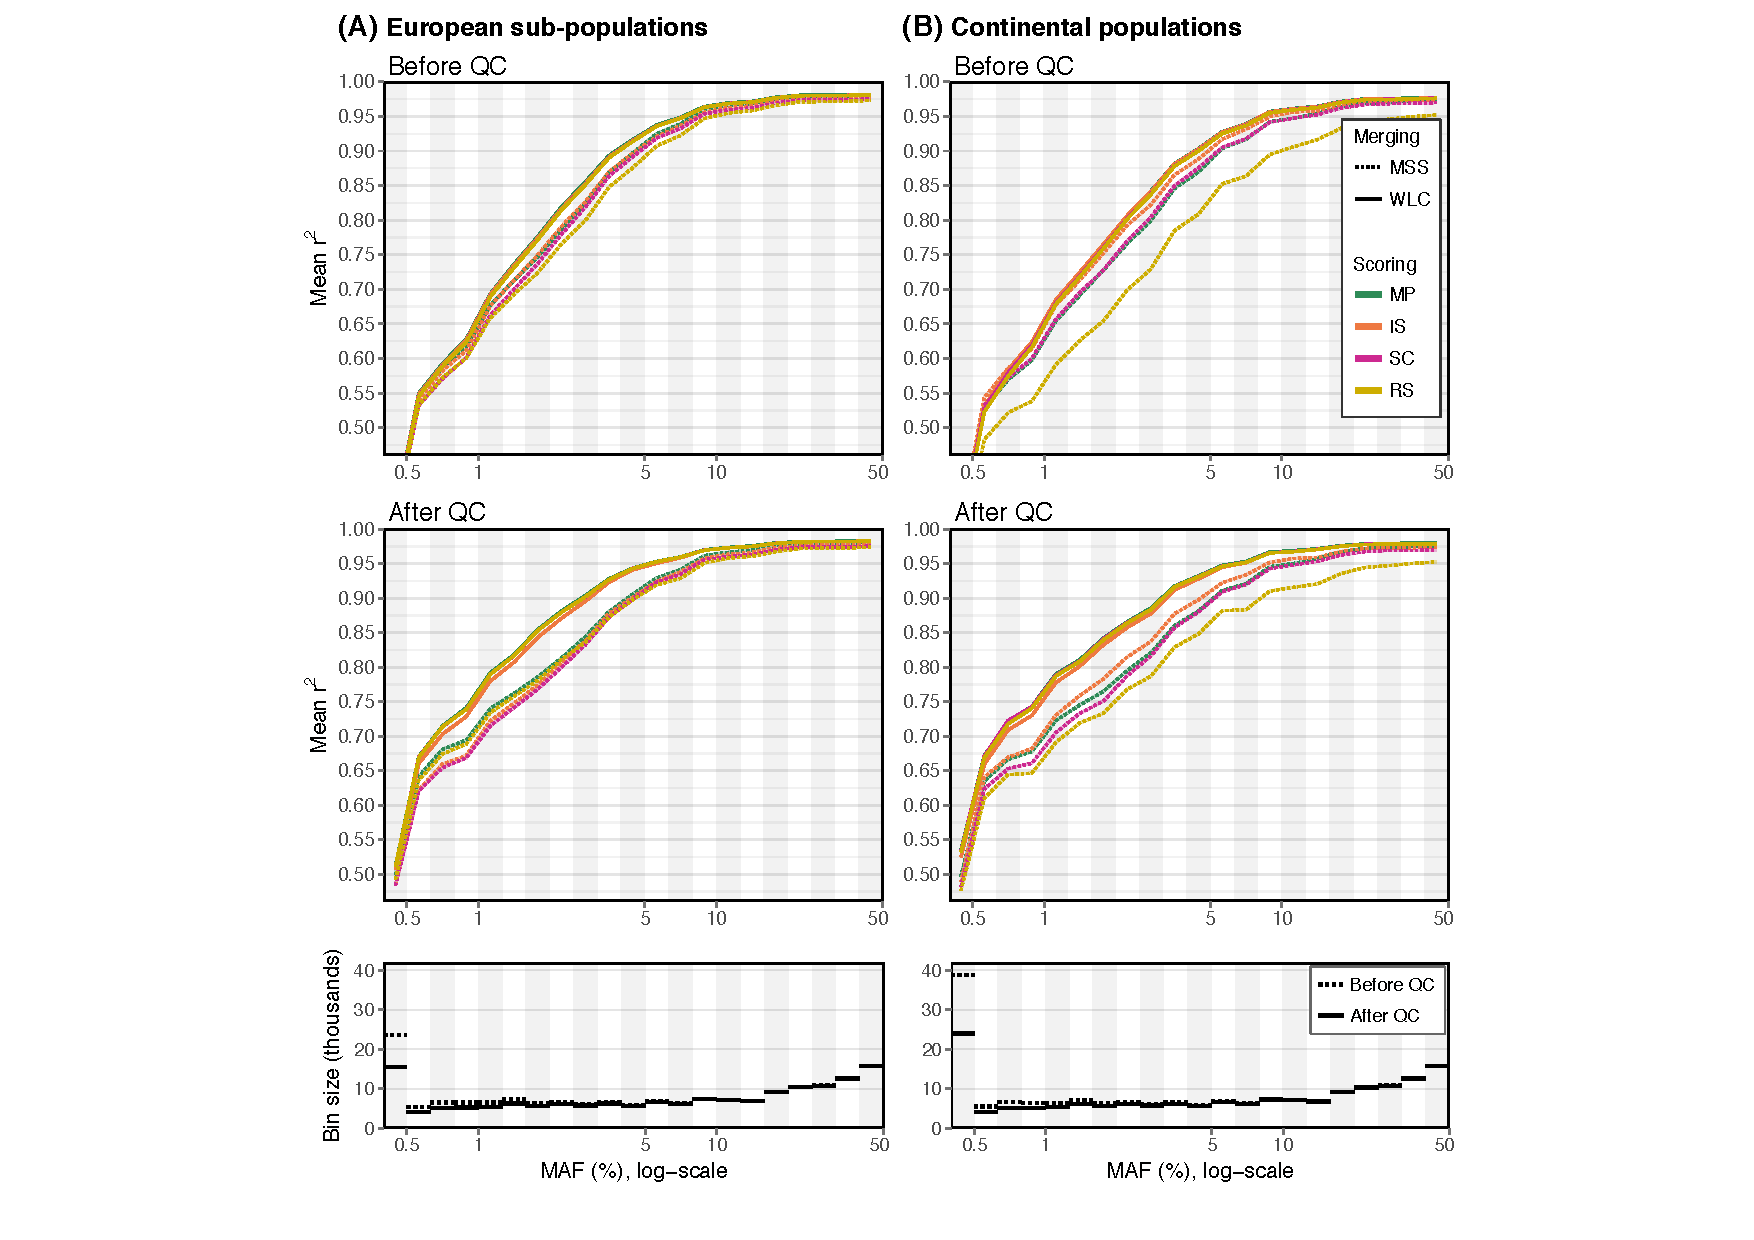
\includegraphics[width=\textwidth]{./img/ch2/accuracy_mim_maf_rsq}
\Caption{Accuracy comparison of score metrics and merge operations in meta-imputation}
{Each combination of merge operation (\texttt{MSS} and \texttt{WLC}) and score metric (\texttt{MP}, \texttt{IS}, \texttt{SC}, and \texttt{RS}) was examined in Scenarios~A and B.
Accuracy was measured as mean~${r^2}$ calculated between meta-imputed variants and variants masked in the \gls{got2d} dataset.
Results are shown both before and after \gls{qc}.
Bin sizes were defined on log-scale where \emph{grey-white} bars indicate boundaries.
The panels at the bottom indicate the number of variants per bin before \gls{qc} (\emph{dotted}) and the average number of variants per bin after \gls{qc} (\emph{solid}).}
{fig:mim_rsq}
\end{figure}

%

Although \texttt{MSS} overall preserved a relatively large proportion of markers after \gls{qc}, the accuracy of retained genotypes was overall lower compared to data produced under \texttt{WLC}.
Imputation accuracy improved after \gls{qc} as illustrated in \cpref{fig:mim_rsq}, which shows mean~$r^2$ calculated in \gls{maf} bins of equal size on log-scale.
The differences among settings were small, in particular among score metrics when \texttt{WLC} was used, but where differences in accuracy become more pronounced after \gls{qc}, which highlighted a clear distinction between merge operations.
Throughout, mean $r^2$ was higher for genotype data produced under \texttt{WLC}.
In Scenario~A, for example, mean~$r^2$ at ${\text{MAF} \leq 1\%}$ before \gls{qc} was
\MeanValue{0.4716920}{0.88645e-03} in \texttt{WLC} and
\MeanValue{0.4644852}{0.89356e-03} in \texttt{MSS}, but showed a larger difference after \gls{qc}, namely
\MeanValue{0.6049897}{1.01002e-03} and
\MeanValue{0.4716920}{0.88645e-03} in \texttt{WLC} and \texttt{MSS}, respectively.
This was also seen in Scenario~B,
where mean~$r^2$ at ${\text{MAF} \leq 1\%}$ was
\MeanValue{0.4275046}{0.79637e-03} and
\MeanValue{0.4177174}{0.81126e-03} before \gls{qc} in \texttt{WLC} and \texttt{MSS}, respectively, as well as
\MeanValue{0.5996758}{0.95121e-03} in \texttt{WLC} and
\MeanValue{0.5482575}{0.91363e-03} in \texttt{MSS} after \gls{qc}.
Accuracy differences between merge operations were more pronounced at higher \gls{maf}; as seen in \cref{fig:mim_rsq}.
For example, at ${\text{MAF} \leq 5\%}$ after \gls{qc}, mean~$r^2$ was
\MeanValue{0.8726145}{0.44164e-03} and
\MeanValue{0.8110458}{0.58041e-03}
in Scenario~A for \texttt{WLC} and \texttt{MSS}, respectively, as well as
\MeanValue{0.8617191}{0.47222e-03} and
\MeanValue{0.7931924}{0.64931e-03} in Scenario~B, respectively.

%
% !TEX root = ../../main.tex


\begin{table}[!htb]
\Caption{Accuracy measured for each meta-imputation setting}
{Accuracy was measured as mean~$r^2$ (${\pm\text{SE}}$) per \gls{maf} bin; defined to reflect average levels of accuracy measured at rare, low-frequency, and common variants.
Reported values were measured after \gls{qc} for each meta-imputation setting (combination of merge operation and score metric), in Scenarios~A and B.
\Addition{Retained variants were intersected across datasets per MAF bin.
The number of SNPs at which mean~$r^2$ was measured, $n$, is reported per scenario below the MAF range.}
The setting with the highest accuracy per \gls{maf} bin and per scenario is highlighted (\textbf{bold}).\CorrectLabel}
{tab:mim_rsq}
\centering
\TableUnits
\begin{threeparttable}
\begin{tabular}{%
	l@{\quad}c@{\quad}c%
	S[table-format=1.3]%
  @{}S[table-format=1.3]%
	S[table-format=1.3]%
	@{}S[table-format=1.3]%
	}
\toprule
{MAF bin} & {Merge} & {Score} &
\multicolumn{2}{c}{Scenario A} &
\multicolumn{2}{c}{Scenario B} \\
\cmidrule(lr){4-5}
\cmidrule(lr){6-7}
 & & & {Mean $r^2$} & {($\pm$~SE$^\ast$)} & {Mean $r^2$} & {($\pm$~SE$^\ast$)} \\
\otoprule
\multirow{3}{*}{\shortstack[l]{{\bfseries[0.00, 0.01]} \\ ~ $n_A = \num{28341}$ \\ ~ $n_B = \num{33443}$}}
 & \texttt{MSS}
  & \texttt{MP} & \bfseries 0.610644 & (2.057332)  &  0.601723 & (1.997402) \\
& & \texttt{IS} &  0.602369 & (2.067987)  &  0.599291 & (2.005439) \\
& & \texttt{SC} &  0.600145 & (2.040775)  &  0.594598 & (1.961289) \\
& & \texttt{RS} &  0.600892 & (2.051666)  &  0.578417 & (1.977409) \\
\cmidrule(lr){3-7}
& \texttt{WLC}
  & \texttt{MP} &  0.609431 & (2.041139)  & \bfseries 0.603334 & (1.957030) \\
& & \texttt{IS} &  0.607690 & (2.042573)  &  0.602691 & (1.958653) \\
& & \texttt{SC} &  0.607655 & (2.038668)  &  0.601475 & (1.951390) \\
& & \texttt{RS} &  0.607538 & (2.038956)  &  0.601114 & (1.951605) \\
\cmidrule(lr){1-7}
\multirow{3}{*}{\shortstack[l]{{\bfseries(0.01, 0.05]} \\ ~ $n_A = \num{38669}$ \\ ~ $n_B = \num{37364}$}}
 & \texttt{MSS}
  & \texttt{MP} &  0.870894 & (0.952739)  &  0.858368 & (1.075501) \\
& & \texttt{IS} &  0.859376 & (1.008176)  &  0.860007 & (1.071849) \\
& & \texttt{SC} &  0.855345 & (0.968571)  &  0.845538 & (1.061551) \\
& & \texttt{RS} &  0.847281 & (1.035284)  &  0.807120 & (1.266720) \\
\cmidrule(lr){3-7}
 & \texttt{WLC}
  & \texttt{MP} & \bfseries 0.879115 & (0.866827)  & \bfseries 0.866884 & (0.956957) \\
& & \texttt{IS} &  0.876414 & (0.877540)  &  0.865731 & (0.961977) \\
& & \texttt{SC} &  0.875809 & (0.876575)  &  0.863791 & (0.961773) \\
& & \texttt{RS} &  0.875685 & (0.876986)  &  0.863342 & (0.962887) \\
\cmidrule(lr){1-7}
\multirow{3}{*}{\shortstack[l]{{\bfseries(0.05, 0.50]} \\ ~ $n_A = \num{92797}$ \\ ~ $n_B = \num{91375}$}}
 & \texttt{MSS}
  & \texttt{MP} &  0.975080 & (0.212736)  &  0.969429 & (0.261345) \\
& & \texttt{IS} &  0.971473 & (0.232792)  &  0.970468 & (0.261916) \\
& & \texttt{SC} &  0.968808 & (0.234113)  &  0.964816 & (0.253617) \\
& & \texttt{RS} &  0.965034 & (0.262540)  &  0.939578 & (0.418136) \\
 \cmidrule(lr){3-7}
 & \texttt{WLC}
  & \texttt{MP} & \bfseries 0.977060 & (0.175426)  & \bfseries 0.973858 & (0.184269) \\
& & \texttt{IS} &  0.976379 & (0.178054)  &  0.973197 & (0.184769) \\
& & \texttt{SC} &  0.976284 & (0.178625)  &  0.972677 & (0.187366) \\
& & \texttt{RS} &  0.976253 & (0.178787)  &  0.972410 & (0.188150) \\
 \bottomrule
 \end{tabular}
 \begin{tablenotes}\footnotesize
 	\item[{${\ast}$}] Standard error (SE) $\times 10^{-3}$
 \end{tablenotes}
 \end{threeparttable}
\end{table}



%
% pre-correction (SNPS were not intersected):
%
% \begin{threeparttable}
% \begin{tabular}{%
% 	l@{\quad}c@{\quad}c%
% 	S[table-format=1.3]%
%   @{}S[table-format=1.3]%
% 	S[table-format=5.0]%
% 	S[table-format=1.3]%
% 	@{}S[table-format=1.3]%
% 	S[table-format=5.0]%
% 	}
% \toprule
% {MAF bin} & {Merge} & {Score} &
% \multicolumn{3}{c}{Scenario A} &
% \multicolumn{3}{c}{Scenario B} \\
% \cmidrule(lr){4-6}
% \cmidrule(lr){7-9}
%  & & & {Mean $r^2$} & {($\pm$~SE$^\ast$)} & {$n$} & {Mean $r^2$} & {($\pm$~SE$^\ast$)} & {$n$} \\
% \otoprule
% {{[0.00, 0.01]}}
%  & \texttt{MSS}
%    & \texttt{MP} &  0.584947 & (1.946525) & 31694  &  0.557479 & (1.822788) & 42101 \\
%  & & \texttt{IS} &  0.567338 & (1.968234) & 32099  &  0.554399 & (1.819030) & 42769 \\
%  & & \texttt{SC} &  0.564983 & (1.952322) & 31646  &  0.544109 & (1.769496) & 42335 \\
%  & & \texttt{RS} &  0.578163 & (1.988586) & 30693  &  0.535900 & (1.900744) & 38468 \\
% \cmidrule(lr){3-9}
%  & \texttt{WLC}
%    & \texttt{MP} & \bfseries 0.607540 & (2.018734) & 28818  & \bfseries 0.603224 & (1.911612) & 35020 \\
%  & & \texttt{IS} &  0.599807 & (2.003624) & 29461  &  0.592187 & (1.869955) & 37049 \\
%  & & \texttt{SC} &  0.606387 & (2.027033) & 28607  &  0.602938 & (1.910916) & 34793 \\
%  & & \texttt{RS} &  0.606362 & (2.030836) & 28545  &  0.600816 & (1.917677) & 34748 \\
% \cmidrule(lr){2-9}
% {{(0.01, 0.05]}}
%  & \texttt{MSS}
%    & \texttt{MP} &  0.818479 & (1.169141) & 43330  &  0.798540 & (1.324721) & 42865 \\
%  & & \texttt{IS} &  0.809187 & (1.168439) & 43787  &  0.813986 & (1.219665) & 43341 \\
%  & & \texttt{SC} &  0.803550 & (1.146422) & 43499  &  0.789748 & (1.231260) & 43570 \\
%  & & \texttt{RS} &  0.813084 & (1.157015) & 41848  &  0.768786 & (1.416076) & 40173 \\
% \cmidrule(lr){3-9}
%  & \texttt{WLC}
%    & \texttt{MP} & \bfseries 0.875631 & (0.870685) & 39309  & \bfseries 0.864771 & (0.936379) & 39240 \\
%  & & \texttt{IS} &  0.866544 & (0.903124) & 40107  &  0.856054 & (0.961843) & 40376 \\
%  & & \texttt{SC} &  0.874198 & (0.878352) & 39000  &  0.863396 & (0.936293) & 38992 \\
%  & & \texttt{RS} &  0.874232 & (0.878709) & 38972  &  0.862837 & (0.940820) & 38943 \\
% \cmidrule(lr){2-9}
% {{(0.05, 0.50]}}
%  & \texttt{MSS}
%  	 & \texttt{MP} &  0.970186 & (0.280056) & 93571  &  0.960115 & (0.372269) & 93068 \\
%  & & \texttt{IS} &  0.966985 & (0.287216) & 93569  &  0.962408 & (0.343832) & 93567 \\
%  & & \texttt{SC} &  0.964351 & (0.287651) & 93541  &  0.955981 & (0.342034) & 93544 \\
%  & & \texttt{RS} &  0.961725 & (0.301301) & 93336  &  0.931022 & (0.488260) & 92876 \\
%  \cmidrule(lr){3-9}
%  & \texttt{WLC}
%  	 & \texttt{MP} & \bfseries 0.976555 & (0.181332) & 92952  & \bfseries 0.972756 & (0.192585) & 92198 \\
%  & & \texttt{IS} &  0.975928 & (0.183156) & 92943  &  0.971667 & (0.195965) & 92435 \\
%  & & \texttt{SC} &  0.976184 & (0.179378) & 92857  &  0.971936 & (0.191300) & 92122 \\
%  & & \texttt{RS} &  0.976165 & (0.179460) & 92852  &  0.971744 & (0.191307) & 92096 \\
%  \bottomrule
%  \end{tabular}
%  \begin{tablenotes}\footnotesize
%  	\item[{${\ast}$}] Standard error (SE) $\times 10^{-3}$
%  \end{tablenotes}
%  \end{threeparttable}

%

Accuracy as measured for each setting after \gls{qc} is given in \cpref{tab:mim_rsq}, which shows mean~$r^2$ computed in \n{3} broader MAF bins to summarise accuracy levels at
rare variants (here defined at ${\text{MAF} \in \left[ 0.00, 0.01\right]}$),
low-frequency (${\text{MAF} \in \left( 0.01, 0.05\right]}$), and
common variants (${\text{MAF} \in \left( 0.05, 0.50\right]}$).
The \texttt{RS} score metric overall resulted in less accurate genotype data compared to other metrics, in particular in Scenario~B where \texttt{RS} was least accurate in all comparisons. This was not the case in Scenario~A, where it showed a higher accuracy than \texttt{IS} and \texttt{SC} at rare and low-frequency variants.
However, note that accuracy differences among score metrics were low overall in Scenario~A (see \cref{tab:mim_rsq}), due to the presumed higher genetic similarity between sample individuals and reference haplotypes (recall that the \gls{got2d} sample is composed of individuals of Central and Northern European descent).

Regardless, \texttt{MP} (maximum probability) outperformed other score metrics in most comparisons; except in Scenario~B, for low-frequency variants under \texttt{MSS}, where it was outperformed by \texttt{IS}.
The \texttt{MP} score metric was found to further improve accuracy under \texttt{WLC}, such that the combination of \texttt{MP} and \texttt{WLC} was seen to yield the highest accuracy in each \gls{maf} bin and in both scenarios (as highlighted in \cref{tab:mim_rsq}).
Therefore, in the following, \texttt{WLC} was chosen as merge operation and \texttt{MP} as score metric; hence, the combination of \texttt{MP} and \texttt{WLC} is implied when referring to meta-imputation below.


%
\subsubsection{Improvements of accuracy in comparison to direct imputations}
%

Available split panels were imputed into the generated study sample and imputed genotype data were then combined through meta-imputation.
The union and intersection panels were separately imputed for subsequent comparison to meta-imputed genotypes.
Before accuracy was measured, all data were subjected to \gls{qc} and variants were removed when not matched to masked variants or when contained in the imputation scaffold.
For simplicity, imputed datasets are referred to by the panel from which they were estimated.

Comparisons were based on mean~$r^2$ calculated at corresponding (meta-)imputed and masked variants pooled by \gls{maf} bin.
In addition, significant differences in the \gls{maf} distribution of imputed and corresponding meta-imputed variants were determined using the \n{2}-sample Kolmogorov–-Smirnov (KS) test.
However, significance was determined from the median of the KS test statistic, here denoted by $\widetilde{D}$, calculated at ${n = \num{500}}$ randomly selected sites over \n{1000} repeated draws.
This was done to account for varying subset sizes retained in each comparison, and to avoid potential biases due to correlations of \gls{ld} at nearby markers.
\Gls{maf} distributions were significantly different if
\begin{equation}\label{eq:meta_ks_test}
	\widetilde{D}_{n} ~ > ~ c(\alpha) \sqrt{\frac{2n}{n^2}}
\end{equation}
for significance levels ${c(0.05)=1.36}$ and ${c(0.01)=1.63}$.
A similar approach was applied by \citet{Pasaniuc:2014hq} to compare signatures of functional enrichment in imputed data.



%
% !TEX root = ../../main.tex


\begin{table}[!htb]
\TableUnits
\Caption{Effect of quality control on imputed genotype data}
{The number (percent) of variants retained after \gls{qc} for direct imputations (\ie \n{4} split panels, intersection panel, and union panel) and meta-imputation. Numbers refer to variants retained after removing unmatched sites and those contained in the imputation scaffold.}
{tab:imp_qc}
\centering
\begin{tabular}{%
	l%
	lS[table-format=6.0]@{\quad}S[round-precision=1,table-format=1.1]%
	lS[table-format=6.0]@{\quad}S[round-precision=1,table-format=1.1]%
	}
\toprule
 Panel & \multicolumn{3}{c}{Scenario A} & \multicolumn{3}{c}{Scenario B} \\
 \cmidrule(lr){2-4}
 \cmidrule(lr){5-7}
 & {Split} & {$n$ retained} & {(\%)} & {Split} & {$n$ retained} & {(\%)} \\
\otoprule
Split panel (1)              & CEU & 135218 & (95.42016) &  AFR & 123662 & (91.84095) \\
Split panel (2)              & FIN & 141017 & (96.60485) &  AMR & 155266 & (93.62115) \\
Split panel (3)              & GBR & 137277 & (94.98166) &  ASN &  99531 & (94.29660) \\
Split panel (4)              & TSI & 138613 & (94.02081) &  EUR & 161364 & (95.34062) \\
\cmidrule(lr){2-4}
\cmidrule(lr){5-7}
Meta-imputed (1--4)          &  -- & 161079 & (88.71894) &   -- & 166458 & (84.79776) \\
\slshape Intersection panel  &  -- & 116980 & (99.80292) &   -- &  92312 & (99.83669) \\
\slshape Union panel         &  -- & 174229 & (95.96169) &   -- & 184158 & (93.81457) \\
\bottomrule
\end{tabular}
\end{table}

%

The numbers of retained variants for each panel are given in \cpref{tab:imp_qc}.
Meta-imputed data showed the highest proportion of variants removed through \gls{qc}.
In Scenario~A, \Percent{11.281057} of meta-imputed variants were removed, whereas only \Percent{0.1970805} of variants in the intersection and \Percent{4.0383122} in the union panel were removed, compared to an average of \MeanPercent{4.743128}{0.5359804} among split panels.
Note that only \Percent{3.3951484} of markers did not pass \gls{qc} after imputation from the FIN sub-population.
The proportion of meta-imputed genotypes removed after \gls{qc} was also highest in Scenario~B (\Percent{15.202241}) which is compared to only \Percent{0.1633086} in the intersection and \Percent{6.1854305} in the union panel, as well as \MeanPercent{6.225171}{0.7352695} on average in split panels, where the lowest proportion of removed variants was seen for the EUR panel (\Percent{4.6593796}).
However, the number of retained variants in meta-imputed data (\num{161076} and \num{166458} in A and B, respectively) exceeded those retained in any split panel or the intersection panel; see \cref{tab:imp_qc}.

%
%!TEX root = ../../main.tex


\begin{figure}[p]
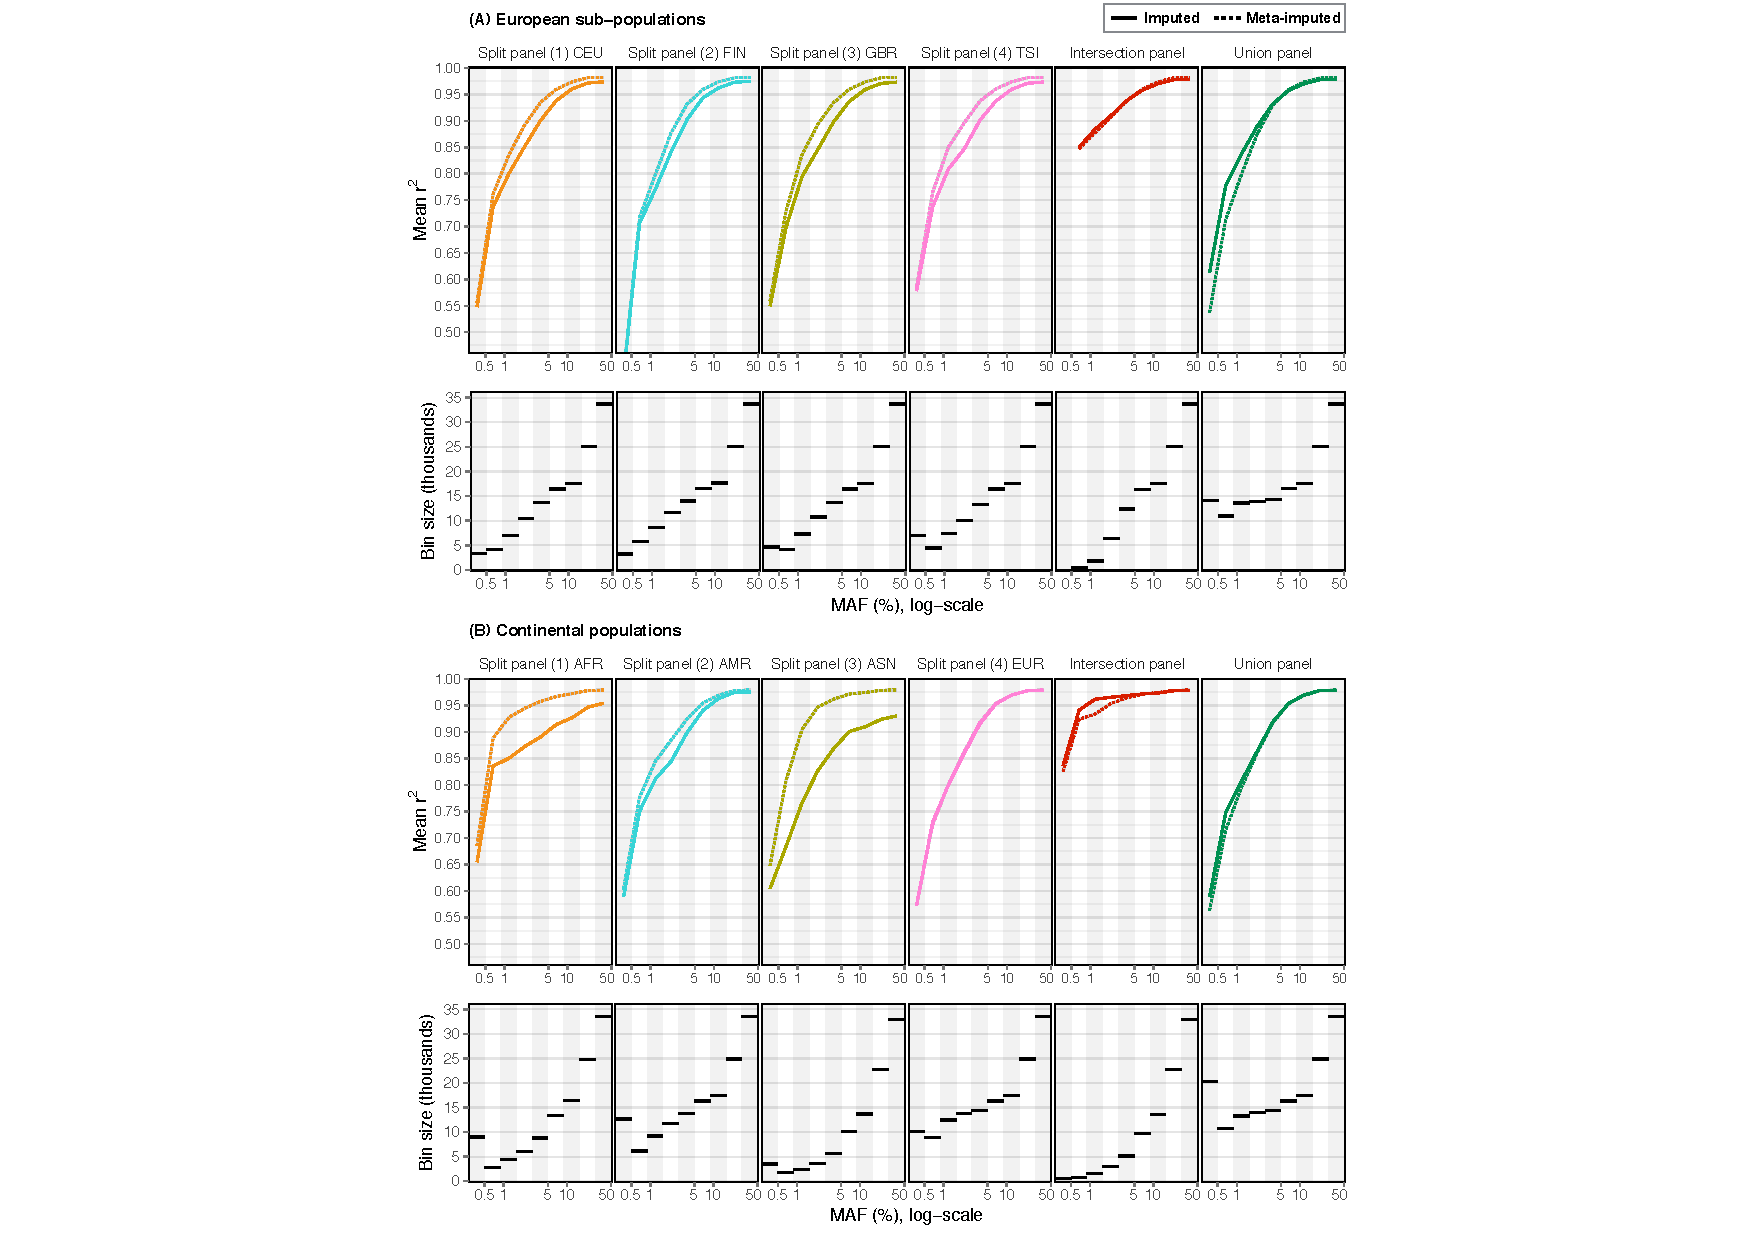
\includegraphics[width=\textwidth]{./img/ch2/accuracy_imp_maf_rsq}
\Caption{Accuracy comparison between meta-imputation and direct imputations}
{Accuracy was measured as mean~$r^2$ per \gls{maf} bin, defined on log-scale where \emph{grey-white} bars indicate boundaries.
Each imputed panel (imputations from the \n{4} split panels, the intersection panel, and the union panel) was separately compared to meta-imputation on the same set of variants per bin \Addition{(\ie on the intersected set of SNPs per comparison)}; shown for variants retained after \gls{qc}, in Scenarios~A and B.
\Gls{maf} bins were defined on the actual allele frequencies as determined by the \gls{got2d} dataset.
Note that mean~$r^2$ is not shown if the number of markers dropped below \n{50} per \gls{maf} bin.
Panels at the bottom show the number of variants compared per bin.}
{fig:imp_rsq}
\end{figure}

%

Each of the imputed datasets was compared separately to meta-imputation, on the same set of variants retained after \gls{qc}.
The distribution of accuracy (mean~$r^2$) measured by \gls{maf} is shown in \cpref{fig:imp_rsq}; average accuracy measured for each imputation strategy in comparison to meta-imputation is given in \cpref{tab:imp_rsq}, where accuracy was measured by \gls{maf} to distinguish
rare variants (${\text{MAF} \in \left[ 0.00, 0.01\right]}$),
low-frequency (${\text{MAF} \in \left( 0.01, 0.05\right]}$), and
common variants (${\text{MAF} \in \left( 0.05, 0.50\right]}$).

In Scenario~A, meta-imputation showed an improvement in accuracy over imputations from split panels.
For example, for rare variants, the highest improvement among split panel comparisons was seen with the GBR sample, where mean~$r^2$ was \MeanValue{0.6366850}{3.37107e-03} for GBR and \MeanValue{0.6589668}{3.29561e-03} for meta-imputed data.
Differences were larger at low-frequency, where the highest improvement was seen in comparison with the TSI sample;
\MeanValue{0.8647786}{1.16400e-03} and \MeanValue{0.9068669}{0.80808e-03}
for TSI and meta-imputation, respectively.
Only the union panel was higher in accuracy than meta-imputation; \eg
\MeanValue{0.6966732}{1.87252e-03} and \MeanValue{0.6266977}{2.00122e-03}
for rare variants, respectively, and
\MeanValue{0.8926102}{0.80090e-03} and \MeanValue{0.8769747}{0.85858e-03}
at low-frequency variants, respectively.
Meta-imputation showed approximately equal levels of accuracy as the union panel at common variants, where the difference in mean~$r^2$ was \MeanValue{0.003182026}{0.811088e-04}.

%
% !TEX root = ../../main.tex


\begin{table}[p]
\Caption{Accuracy of imputation strategies at rare, low-frequency, and common variants}
{Accuracy was calculated as mean~$r^2$ per \gls{maf} bin on the same set of variants retained after \gls{qc} in each comparison between meta-imputation and direct imputation, where $n$ denotes the number of variants compared.
The imputation strategy with the highest accuracy is highlighted (\textbf{bold}).
The median of KS test statistic, $\widetilde{D}_{500}$, determined whether imputed and meta-imputed \gls{maf} distributions were significantly different; see \ctref{eq:meta_ks_test}.}
{tab:imp_rsq}
\centering
\TableUnits
\begin{threeparttable}
\begin{tabular}{%
	ll%
	S[table-format=5.0]%
  S[table-format=1.3]@{}S[table-format=1.3]%
  S[table-format=1.3]@{}S[table-format=1.3]%
	S[table-format=1.3,table-align-text-post=false,table-space-text-post={*}]
	}
\toprule
{MAF bin} & {Panel} & {$n$} &
\multicolumn{2}{c}{Imputation} &
\multicolumn{2}{c}{Meta-imputation} &
{KS test$^\dagger$} \\
\cmidrule(lr){4-5}
\cmidrule(lr){6-7}
 & & & {Mean $r^2$} & {($\pm$~SE$^\ddagger$)} & {Mean $r^2$} & {($\pm$~SE$^\ddagger$)} & {$\widetilde{D}_{500}$} \\
\otoprule
\multicolumn{8}{@{ }l}{\textbf{Scenario A}\quad(European sub-populations)} \\
\midrule
{{[0.00, 0.01]}}
 & Split panel, CEU &  8636  &  0.664810 & (3.491492)  & \bfseries 0.683215 & (3.401931) & 0.046 \\
 & Split panel, FIN & 10416  &  0.619024 & (3.291918)  & \bfseries 0.629806 & (3.255431) & 0.024 \\
 & Split panel, GBR & 10023  &  0.636685 & (3.371077)  & \bfseries 0.658966 & (3.295617) & 0.034 \\
 & Split panel, TSI & 12763  &  0.653711 & (2.973932)  & \bfseries 0.670288 & (2.909213) & 0.098* \\
 \cmidrule(lr){3-8}
 & \slshape Intersection panel &   546  &  0.822921 & (9.901204)  & \bfseries 0.823535 & (9.831856) & 0.028 \\
 & \slshape        Union panel & 27712  & \bfseries 0.696673 & (1.872524)  &  0.626697 & (2.001220) & 0.264** \\
\cmidrule(lr){2-8}
{{(0.01, 0.05]}}
 & Split panel, CEU & 30012  &  0.865500 & (1.091816)  & \bfseries 0.902455 & (0.812636) & 0.040 \\
 & Split panel, FIN & 32969  &  0.853442 & (1.076218)  & \bfseries 0.885026 & (0.887284) & 0.032 \\
 & Split panel, GBR & 30442  &  0.860141 & (1.119440)  & \bfseries 0.901463 & (0.813331) & 0.036 \\
 & Split panel, TSI & 29445  &  0.864778 & (1.164005)  & \bfseries 0.906866 & (0.808084) & 0.036 \\
 \cmidrule(lr){3-8}
 & \slshape Intersection panel & 20604  & \bfseries 0.924906 & (0.849920)  &  0.923345 & (0.803135) & 0.034 \\
 & \slshape        Union panel & 39213  & \bfseries 0.892610 & (0.800904)  &  0.876974 & (0.858581) & 0.088* \\
\cmidrule(lr){2-8}
{{(0.05, 0.50]}}
 & Split panel, CEU & 92885  &  0.964461 & (0.268998)  & \bfseries 0.976659 & (0.180477) & 0.014 \\
 & Split panel, FIN & 92936  &  0.966423 & (0.249706)  & \bfseries 0.976583 & (0.181070) & 0.012 \\
 & Split panel, GBR & 92845  &  0.963589 & (0.273313)  & \bfseries 0.976622 & (0.180833) & 0.012 \\
 & Split panel, TSI & 92840  &  0.963894 & (0.283242)  & \bfseries 0.976786 & (0.179558) & 0.012 \\
 \cmidrule(lr){3-8}
 & \slshape Intersection panel & 92751  &  0.973344 & (0.211934)  & \bfseries 0.976723 & (0.180231) & 0.012 \\
 & \slshape        Union panel & 92938  &  0.973373 & (0.211659)  & \bfseries 0.976555 & (0.181358) & 0.012 \\
 \otoprule
 \multicolumn{8}{@{ }l}{\textbf{Scenario B}\quad(Continental populations)} \\
 \midrule
 {{[0.00, 0.01]}}
  & Split panel, AFR & 12495  &  0.703450 & (3.238338)  & \bfseries 0.744594 & (3.070404) & 0.030 \\
  & Split panel, AMR & 20416  &  0.653123 & (2.479939)  & \bfseries 0.672060 & (2.387583) & 0.040 \\
  & Split panel, ASN &  5661  &  0.639974 & (4.971557)  & \bfseries 0.713699 & (4.585839) & 0.082 \\
  & Split panel, EUR & 21223  & \bfseries 0.658367 & (2.226543)  &  0.656284 & (2.207200) & 0.048 \\
  \cmidrule(lr){3-8}
  & \slshape Intersection panel &  1364  & \bfseries 0.907201 & (4.420106)  &  0.891806 & (4.430467) & 0.172** \\
  & \slshape        Union panel & 33430  & \bfseries 0.653383 & (1.871343)  &  0.626010 & (1.894104) & 0.148** \\
 \cmidrule(lr){2-8}
 {{(0.01, 0.05]}}
  & Split panel, AFR & 18468  &  0.879161 & (1.631274)  & \bfseries 0.948322 & (0.766896) & 0.048 \\
  & Split panel, AMR & 33093  &  0.860770 & (1.157715)  & \bfseries 0.893814 & (0.855185) & 0.036 \\
  & Split panel, ASN & 11181  &  0.836930 & (2.413587)  & \bfseries 0.947709 & (0.953756) & 0.114** \\
  & Split panel, EUR & 38417  & \bfseries 0.867048 & (0.968714)  &  0.869536 & (0.909904) & 0.032 \\
  \cmidrule(lr){3-8}
  & \slshape Intersection panel &  9443  & \bfseries 0.967004 & (0.810571)  &  0.956752 & (0.815682) & 0.062 \\
  & \slshape        Union panel & 39140  & \bfseries 0.870742 & (0.948816)  &  0.866276 & (0.923712) & 0.058 \\
 \cmidrule(lr){2-8}
 {{(0.05, 0.50]}}
  & Split panel, AFR & 88152  &  0.941104 & (0.425965)  & \bfseries 0.976002 & (0.172260) & 0.022 \\
  & Split panel, AMR & 92144  &  0.966958 & (0.263392)  & \bfseries 0.972889 & (0.191426) & 0.016 \\
  & Split panel, ASN & 79581  &  0.921305 & (0.518841)  & \bfseries 0.977514 & (0.165172) & 0.024 \\
  & Split panel, EUR & 92188  &  0.972060 & (0.217795)  & \bfseries 0.972762 & (0.192505) & 0.016 \\
  \cmidrule(lr){3-8}
  & \slshape Intersection panel & 79051  &  0.976452 & (0.201266)  & \bfseries 0.977380 & (0.167886) & 0.016 \\
  & \slshape        Union panel & 92187  & \bfseries 0.972790 & (0.213868)  &  0.972755 & (0.192606) & 0.016 \\
\bottomrule
\end{tabular}
\begin{tablenotes}\footnotesize
	\item[{${\dagger}$}] Median of the Kolmogorov–Smirnov (KS) test statistic, $\widetilde{D}$; empirical CDF of imputed and meta-imputed \gls{maf} tested at ${\alpha = 0.05}$ ($\ast$) and ${\alpha = 0.01}$ (${\ast\ast}$).
	\item[{${\ddagger}$}] Standard error (SE) $\times 10^{-3}$.
\end{tablenotes}
\end{threeparttable}
\end{table}

%

Genotype accuracy showed higher differences in Scenario~B, where meta-imputation improved accuracy in most split panel comparisons.
For rare variants, the highest difference was seen to genotype data imputed from the AFR split panel, where mean~$r^2$ was \MeanValue{0.7034507}{3.23833e-03}, compared to \MeanValue{0.7445944}{3.07040e-03} for meta-imputed genotypes.
However, meta-imputation showed similar accuracy as the imputation from the EUR sample, where the difference in mean~$r^2$ was \MeanValue{0.002083192}{0.715902e-04}.
Likewise, at low-frequency, mean~$r^2$ was \MeanValue{0.879161}{1.63127e-03} for AFR and \MeanValue{0.948322}{0.76689e-03} for meta-imputation, and the difference in accuracy was \MeanValue{0.002487}{0.36658e-03} with regard to the EUR split panel.
As in Scenario~A, differences were smaller for common variants, such that the difference in mean~$r^2$ was below \dec{0.001} in comparisons to imputations from the AFR, AMR, and EUR panels, but where the ASN sample showed the highest difference; mean~$r^2$ was \MeanValue{0.921305}{0.51884e-03} for ASN and \MeanValue{0.977514}{0.16517e-03} for meta-imputation.
The union panel was similar in accuracy as meta-imputation, where the overall difference in mean~$r^2$ was \MeanValue{0.01062464}{8.471535e-03}.

Imputations from the intersection panel in Scenario~A and B showed approximately equal levels of accuracy to meta-imputation.
The difference in mean~$r^2$ averaged to \MeanValue{0.0008106733}{1.429231e-04} across \gls{maf} in Scenario~A, and \MeanValue{0.008239279}{4.8183e-03} in Scenario~B.
However, note that the number of variants in the intersection panel was the lowest among available panel data in both scenarios (\cref{tab:imp_qc}), and was further reduced as accuracy was measured on the same sets of variants retained in both the intersection and the meta-imputed datasets.
For example, the comparison between the intersection panel and meta-imputation included only \n{546} variants at \gls{maf} ${\leq 1\%}$ in Scenario~A and \n{1364} variants in Scenario~B, whereas each split panel and the union panel were compared on several thousands of variants at this frequency range.
The high accuracy of genotypes imputed from the intersection panel may result from retaining only those variants that are ``cosmopolitan'' within the scope of the present evaluation.


%
%!TEX root = ../../main.tex


\begin{figure}[!htb]
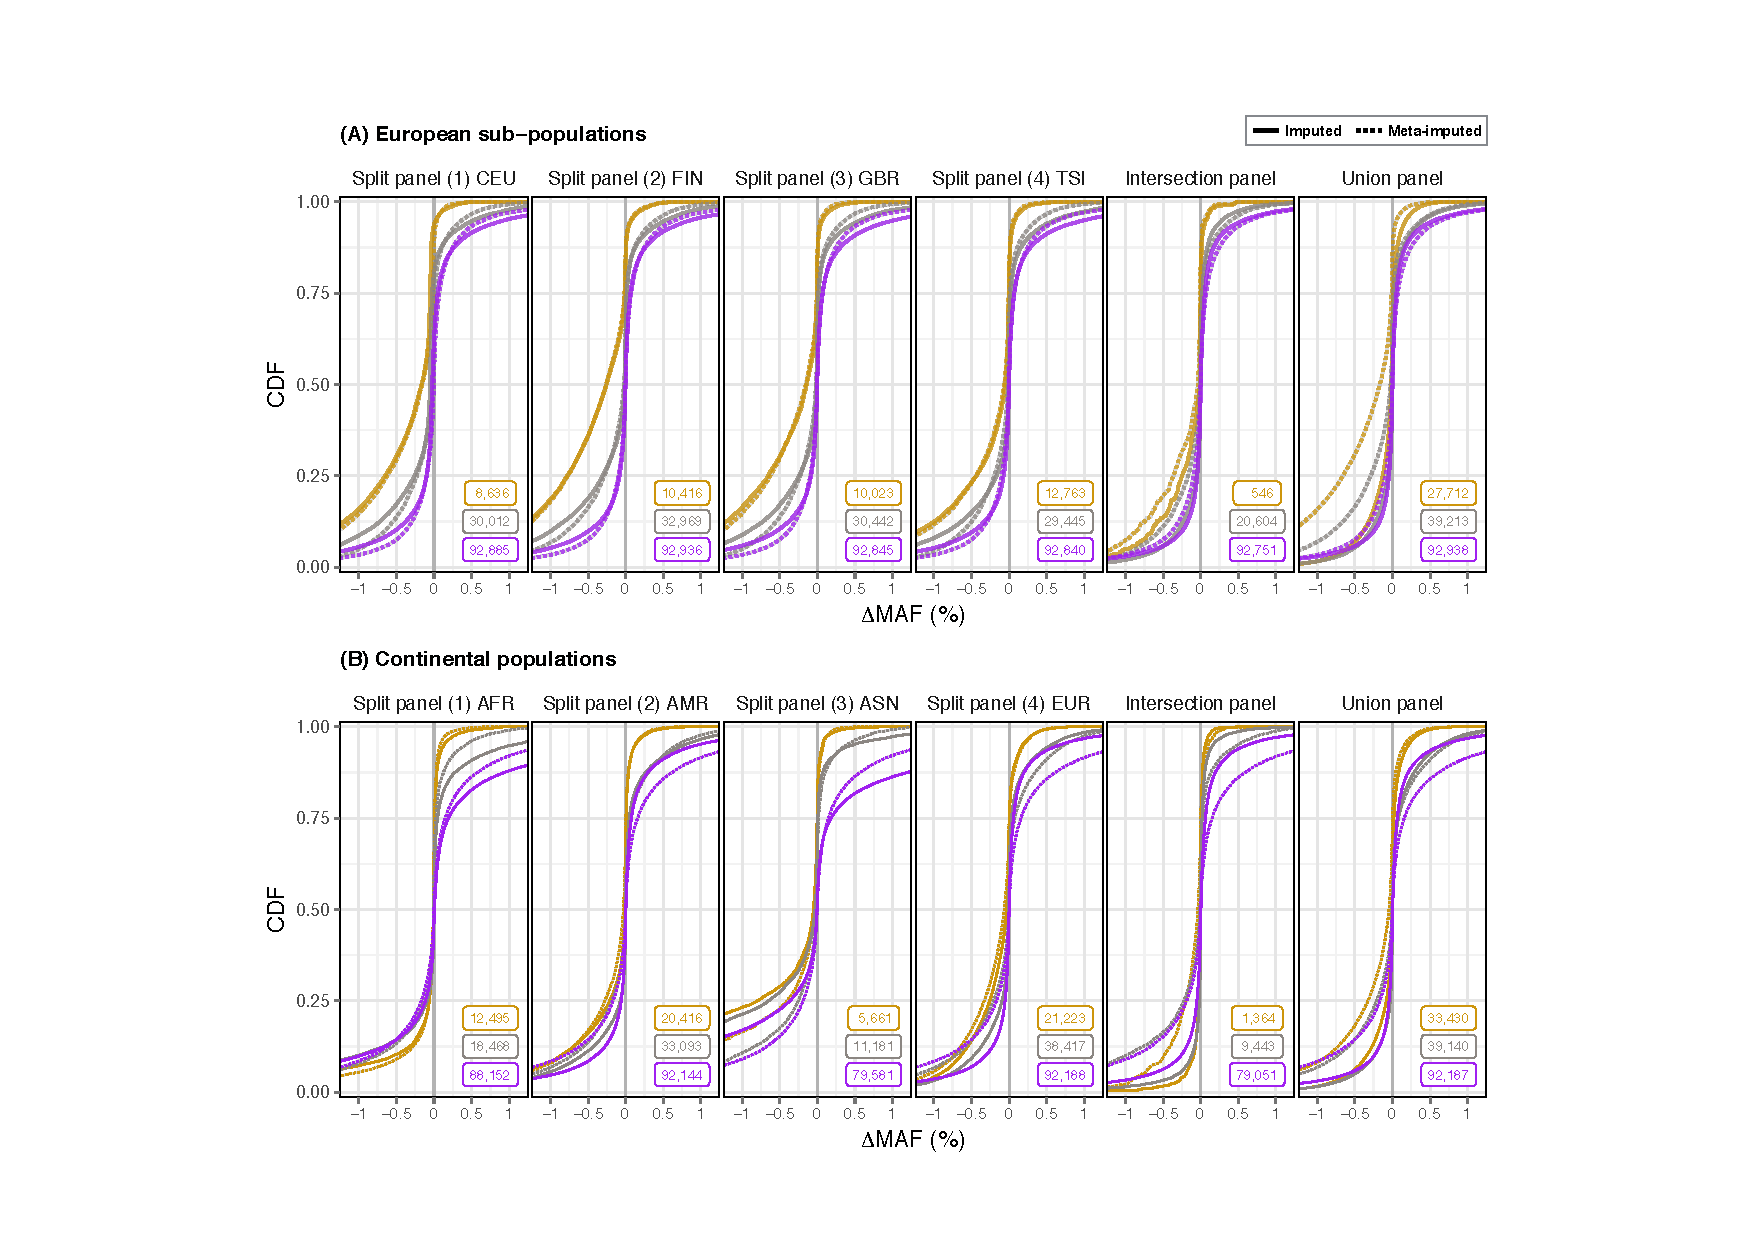
\includegraphics[width=\textwidth]{./img/ch2/accuracy_imputed_delta}
\Caption{Difference between imputed and masked minor allele frequency}
{Comparison of imputed and meta-imputed \gls{maf} in relation to known population frequencies, compared on the same set as retained after \gls{qc} in each comparison.
Frequency difference, ${\Delta\text{MAF}}$, was calculated as the \gls{maf} observed at a masked variant minus \gls{maf} at the corresponding (meta-)imputed variant, pooled in \n{3} \gls{maf} bins; rare variants (${\text{MAF} \in \left[ 0.00, 0.01\right]}$; \emph{yellow}), low-frequency (${\text{MAF} \in \left( 0.01, 0.05\right]}$; \emph{grey}), and common variants (${\text{MAF} \in \left( 0.05, 0.50\right]}$; \emph{purple}).
Numbers per \gls{maf} bin per comparison are given in each panel (\emph{colour-coded}).}
{fig:imp_delta}
\end{figure}

%

Further, the empirical \gls{cdf} of \gls{maf} at imputed and meta-imputed variants was compared per \gls{maf} bin.
Differences are illustrated in \cpref{fig:imp_delta}, which shows the \gls{cdf} of compared variants in relation to the known population frequencies at masked variants in the \gls{got2d} dataset; calculated by subtracting (meta-)imputed frequencies from masked frequencies (${\Delta\text{MAF}}$) at the same set of markers.
Notably, meta-imputed frequencies showed high consistency with imputed frequencies at rare variants (${\text{MAF} \in \left[ 0.00, 0.01\right]}$) across split panel imputations, but were skewed in comparison to imputations from the union panel in both scenarios.
Significant differences were found for rare variant imputations from the TSI sample (${\widetilde{D}=0.098}$) in Scenario~A, as well as for the union panel at rare and low-frequency variants (\dec{0.264} and \dec{0.088}, respectively).
In Scenario~B, imputed and meta-imputed differences were significantly different for rare variant imputations from the intersection panel and the union panel (\dec{0.172} and \dec{0.148}, respectively) and for the union panel at low-frequency variants (\dec{0.114}).
These results suggested that meta-imputation was able to correctly reproduce realistic allele frequency distributions from the combination of imputed genotypes from different sources, while achieving higher or similar accuracy compared to direct imputations from split panels.
Results of KS tests in each comparison are given in \cpref{tab:imp_rsq}.


In summary, split panel imputations were either outperformed or similar levels of accuracy were achieved in direct comparisons to meta-imputed data; see \cref{tab:imp_rsq} for a complete summary of genotype accuracy measured in each comparison.
Although imputations from the union panel outperformed meta-imputation, such differences may be expected given that the union panel contained all the information which meta-imputation had to leverage indirectly from several data sources.
Nonetheless, the present evaluation of genotype accuracy was limited with regard to coverage; for instance, genotype data imputed from the intersection panel was found to be relatively high in accuracy and similar with regard to meta-imputed data, but the low number of variants present in the intersection panel may not yield similar improvements under realistic conditions in association analyses.
Therefore, to provide a comprehensive assessment of the meta-imputation method and to account for a potential tradeoff between accuracy and coverage, I conducted a more extensive power analysis in the following section.



%
\section{Power to detect significant risk signals}
\label{sec:metaimpute_power}
%

The power of meta-imputation to detect disease risk factors in association tests was evaluated using simulated sample data.
This was done in consideration of expected power when causal risk factors vary in their allele frequency as well as risk effect size.
In particular, a series of simulated case-control association experiments was conducted, from which the power to detect significant association signals was determined, at specified allele frequencies and effect size of simulated risk factors.
The description of the methods used is provided below (\ccref{sec:meta_power_methods}), followed by the presentation of results (\ccref{sec:meta_power_results}).


%
\subsection{Methods}
\label{sec:meta_power_methods}
%

The same regime to carry out imputation and \gls{qc} was followed as described in \cpref{sec:meta_accuracy_methods}.
An additional set of haplotype reference data was available from \n{4} independent sequencing studies, which were included here as Scenario~C; see below.
\begin{description}
	\item[Finns.] A Finnish cohort composed of data from the Sequencing Initiative Suomi Project (\emph{SISu}) and the \emph{Finrisk} Project \citep{Vartiainen:2010eb,Pajunen:2010ft,Lim:2014ir,Borodulin:2015bs}; 4x depth; sample size and number of \glspl{snp} considered here were ${N=\num{1941}}$ and ${M=\num{283654}}$, respectively.
	\item[GoNL.] The Genome of the Netherlands Project \citep{Boomsma:2013hf, Deelen:2014dq, GenomeoftheNetherlandsConsortium:2014gs}; 12x depth, consisting of a representative sample of \n{250} trio-families; ${N=\num{748}}$, ${M=\num{362694}}$.
	\item[ORCADES.] The Orkney Complex Disease Study of genetic epidemiology of an isolated population in northern Scotland \citep{McQuillan:2008fz}; 4x depth, family-based data; ${N=\num{399}}$, ${M=\num{236755}}$.
	\item[UK10K.] The \emph{UK10K} Genome Sequencing Project \citep{UKKConsortium:2015ii}; 6.5x depth; ${N=\num{3642}}$, ${M=\num{527199}}$.
\end{description}
Also, an intersection panel was prepared from these \n{4} datasets, but no union panel.
As before, only data from chromosome~20 were considered.
Note that the above datasets were part of the early stage \gls{hrc} testing phase \citep{McCarthy:2016gs}.\footnote{Acknowledgement: Data provided by Professor Jonathan Marchini, Department of Statistics, University of Oxford; prior to the release of the \gls{hrc} dataset.}


%
\subsubsection{Simulation of study sample data}
%

Simulations were performed using \texttt{HAPGEN} version~2.2.0 \citep{Su:2011km}, which requires a \emph{template} dataset of haplotypes to reproduce realistic variant data in \gls{hwe}, such that \gls{ld} patterns in the simulated dataset are consistent with the haplotype sample.
Individual sites can be simulated to independently act as causal disease variants with specified relative risk.
The simulation generates \n{2} \gls{gwa} samples of individuals that are affected (\emph{cases}) or not affected (\emph{controls}) by a disease phenotype.
Data are identical in coverage as the template dataset.

Here, simulations were performed using \gls{got2d} data (chromosome~20) to serve as the template dataset.
The size of simulated case and control samples was fixed to \n{2500} individuals each.
Although a larger sample would have been beneficial in terms of signal detection through association testing, exceeding the size of the template dataset (${N=\num{2657}}$) was expected to result in factitious allele frequency changes.
For example, an iterative re-sampling strategy could be applied to introduce new low-frequency variants \citep[\eg following][]{Moutsianas:2015jm}.
However, this was not done here because the effect size of risk variants (as defined during simulation) would likely be affected by such a sampling process.

A series of simulation experiments was conducted in which \n{1} variant was selected per simulation to act as a causal risk factor.
Its relative risk (RR) was defined for heterozygous genotypes ($RR_{het}$) in a log-additive disease model (\ie multiplicative on linear scale); the following \n{3} risk categories were defined.
\begin{align*}
	\textit{Low risk}     : & \quad {RR_{het}=1.2} \quad {(RR_{hom}=1.44)} \\
	\textit{Modest risk}  : & \quad {RR_{het}=1.6} \quad {(RR_{hom}=2.56)} \\
	\textit{High risk}    : & \quad {RR_{het}=2.0} \quad {(RR_{hom}=4.00)}
\end{align*}
The analysis was performed by conducting \n{300} replicate simulations per risk category, where variants occurring at different frequencies were selected in \n{3} defined \gls{maf} intervals;
very low frequency (${\text{MAF} \in [0.5, 1]\,\%}$), low frequency (${\text{MAF} \in (1, 5]\,\%}$), and high frequency (${\text{MAF} \in (5, 50]\,\%}$), such that \n{100} variants were drawn from each interval and simulated as risk variants.

Note that variant selection was done at random, regardless of presence or absence of the selected variant in any of the available reference panels, so as to mirror conditions encountered under realistic \gls{gwa} settings; \ie when a causal variant itself is absent in an imputation reference, its risk effects may be detectable through \gls{ld} at neighbouring sites.

%
% !TEX root = ../../main.tex


\begin{figure}[!htb]
\centering
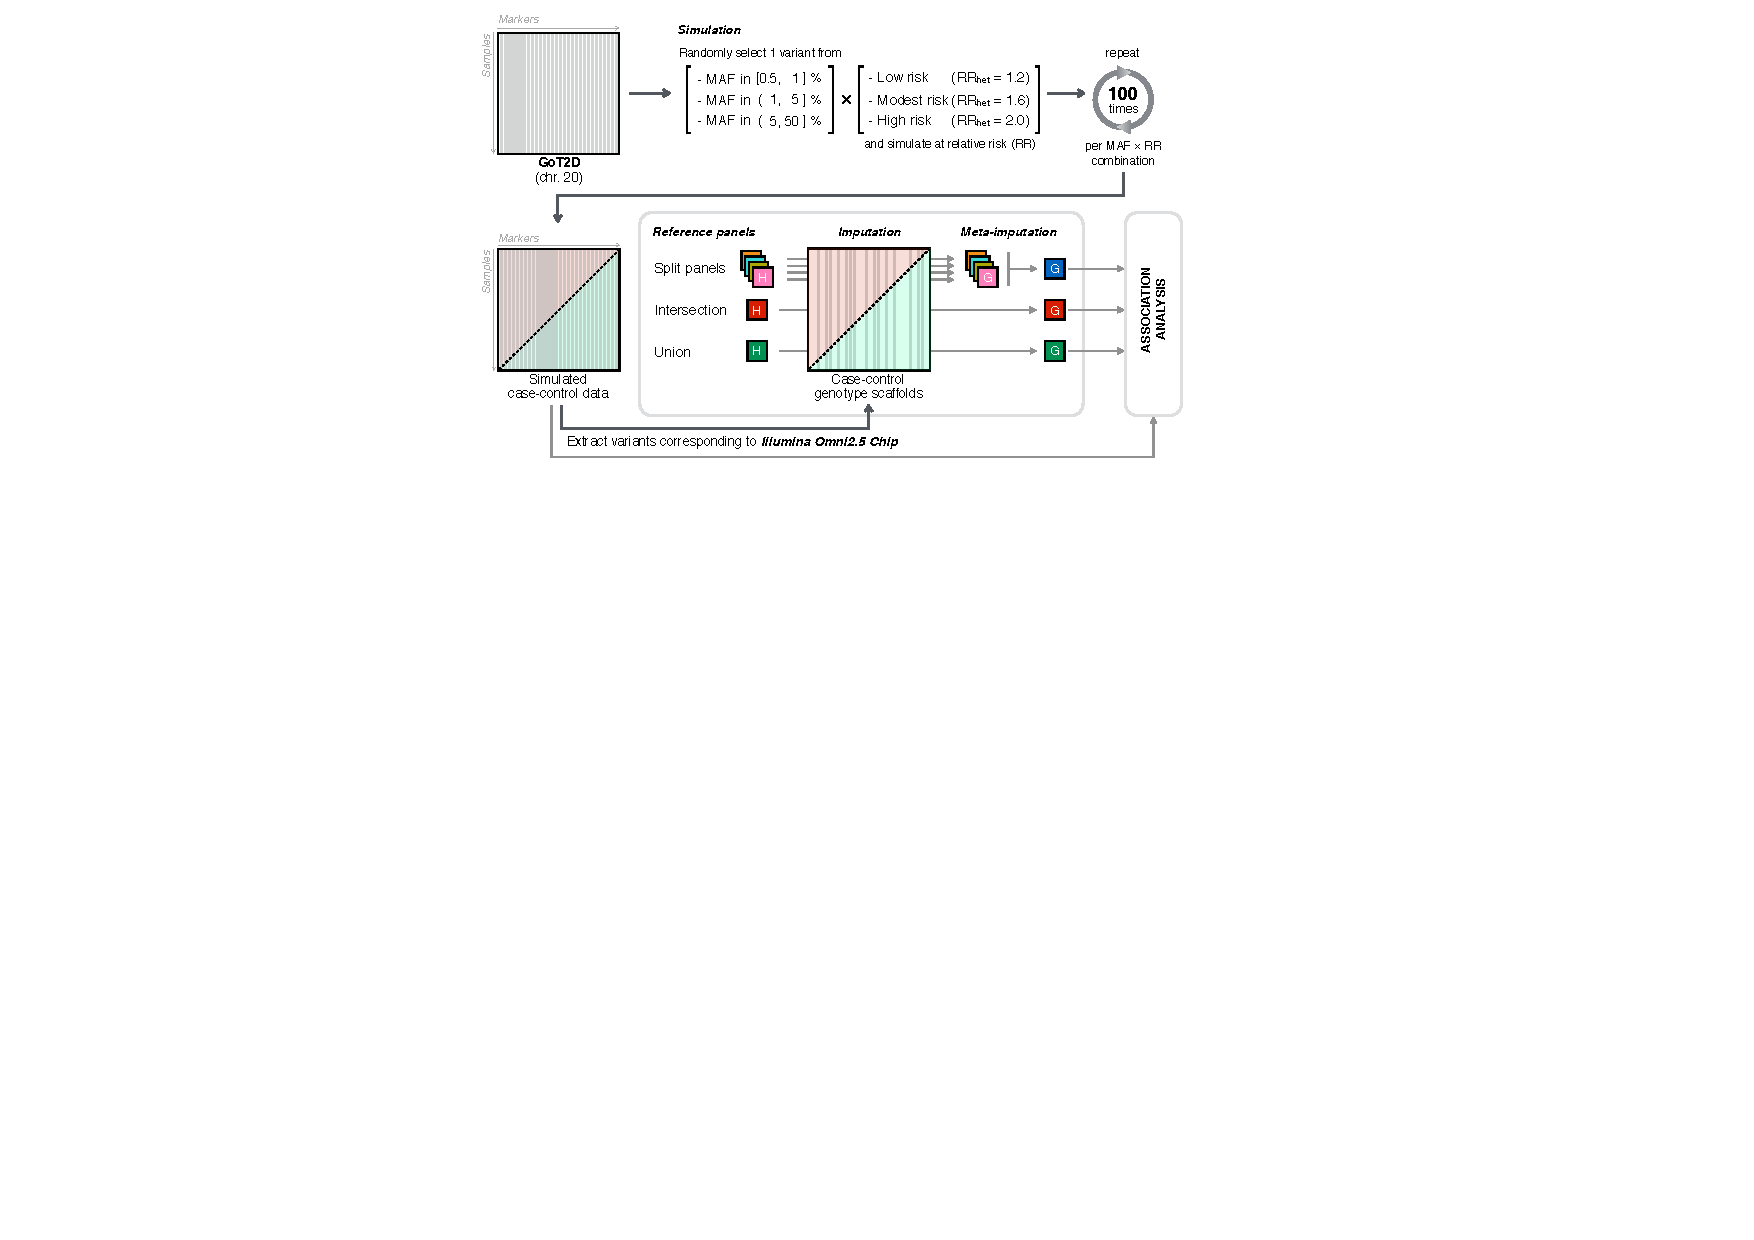
\includegraphics[width=0.9\textwidth]{./img/ch2/info_design_power}
\Caption{Illustration of the simulation process}
{Meta-imputation was assessed in terms of statistical power to detect significant risk association signals in a series of simulated case-control experiments.
The \gls{got2d} dataset was used as a template for simulations using \texttt{HAPGEN} \citep{Su:2011km}, where \n{1} variant was randomly selected within \n{1} of \n{3} defined \gls{maf} intervals.
The selected variant was then simulated to act as a causal disease variant in the simulated case-control dataset, where relative risk ($RR_{het}$) was defined according to \n{1} of \n{3} defined risk categories.
In total, \n{100} replicate simulations were conducted per combination of \gls{maf} interval and risk category (per scenario).
Simulated data were used to extract a genotype scaffold into which available reference panels were imputed, followed by meta-imputation of imputed datasets.
Imputed and meta-imputed datasets were then subjected to association analysis, including the simulated (not imputed) datasets for comparison.}
{fig:info_design_power}
\end{figure}

%

To generate a study sample for imputations, a variant scaffold was extracted from each simulation replicate.
Because the set of simulated variants mirrored those in the \gls{got2d} dataset,
sites that matched with variants typed on \emph{Illumina Omni2.5 Array} were identified and extracted.
A scaffold thus contained \n{40255} variants into which available reference panels were imputed.
Note that simulations produced \n{2} datasets; \n{1} case and \n{1} corresponding control dataset.
These were concatenated before imputation to ensure consistency in the imputation analysis.
Imputed data were again separated into case and control samples prior to association analysis (described below).
Because \texttt{HAPGEN2} produces haplotype data, imputations were executed on pre-phased genotypes.
A summary of the simulation process is illustrated in \cpref{fig:info_design_power}.



%
\subsubsection{Association analysis in imputed genotype data}
%

Imputed case and control datasets were analysed using a frequentist score test under an additive model of association, implemented in \texttt{SNPTEST} version~2.5 \citep{Marchini:2007bg}.
In contrast to the previous analysis (\ctref{metaimpute_accuracy}), in which the variants not included in the extracted scaffold were masked to measure accuracy after imputation, here, the simulated case-control dataset was retained and separately examined in association analysis.
This was done to enable comparisons of meta-imputed and imputed data to a non-imputed benchmark result for each simulation replicate.

The genomic control inflation factor, $\lambda_\text{GC}$, was calculated to investigate if systematic biases are present in association results, which is defined as the median of $\chi^2$~test statistics resulting from case-control association tests divided by the expected median of the $\chi^2$~distribution \citep{Devlin:2001ga}.
Because the frequentist score test was used, $\lambda_\text{GC}$ was calculated on basis of the resulting \pvalues from which the $\chi^2$~statistic was calculated with \n{1} degree of freedom.


%
\subsubsection{Calculation of power in replicate simulation experiments}
%

Significant association signals were identified in each simulation and pooled by \gls{maf} interval and risk category, according to which variants were selected and simulated.
The proportion of datasets in which significance was reached at the known risk variant was taken as a simple estimate for the statistical power to detect genetic risk effects.
Note that the position of the simulated risk variant was known through simulation, but the variant itself may not be retained after imputation or \gls{qc}.
Therefore, signal detection was performed within a 1~\gls{Mb} region around the position of the simulated risk variant, for any site reaching significance with this region.

Significance was defined at a nominal threshold of ${\pvalue\leq1\times10^{-6}}$.
Note that this threshold is higher (thus, less conservative) than commonly applied genome-wide thresholds, \eg at \num{5e-8} \citep[\eg, see][]{Risch:1996ub}, because analyses were conducted on data from chromosome 20 only.
However, to provide additional detail, power was estimated under a moving significance threshold; between ${\pvalue\leq1\times10^{-8}}$ and ${\pvalue\leq1\times10^{-4}}$.
As a comparative measure between association results produced from the different imputation strategies,
the difference in power between the non-imputed simulation dataset and a given (meta-)imputed dataset is reported, denoted by ${\Delta_P}$, which is calculated as the average difference along the moving significance threshold.


%
\subsection{Results}
\label{sec:meta_power_results}
%

A number of \n{100} variants were selected per \gls{maf} interval such that there were 300 variants in total.
Each was then simulated at the \n{3} defined risk categories such that \n{900} simulations were conducted
from which a genotype scaffold was extracted for imputation.
Given the \n{4} split panels, the intersection panel, and the union panel available per Scenario~A and B, as well as the \n{4} independent reference datasets and the generated intersection panel in Scenario~C, a total of \n{15300} imputation analyses were performed.
Imputed data were then combined in meta-imputation (except the intersection and union panels), resulting in \n{900} additional genotype datasets.
Each dataset was then subjected to association analysis, including the non-imputed simulated case-control sample, which was used as a benchmark for comparisons.
Hence, a total of \n{17100} association analyses were conducted, where each was treated as an independent \gls{gwa} study.
All analyses were performed on whole-chromosome data (chromosome~20).


%
%!TEX root = ../../main.tex


\begin{figure}[!htb]
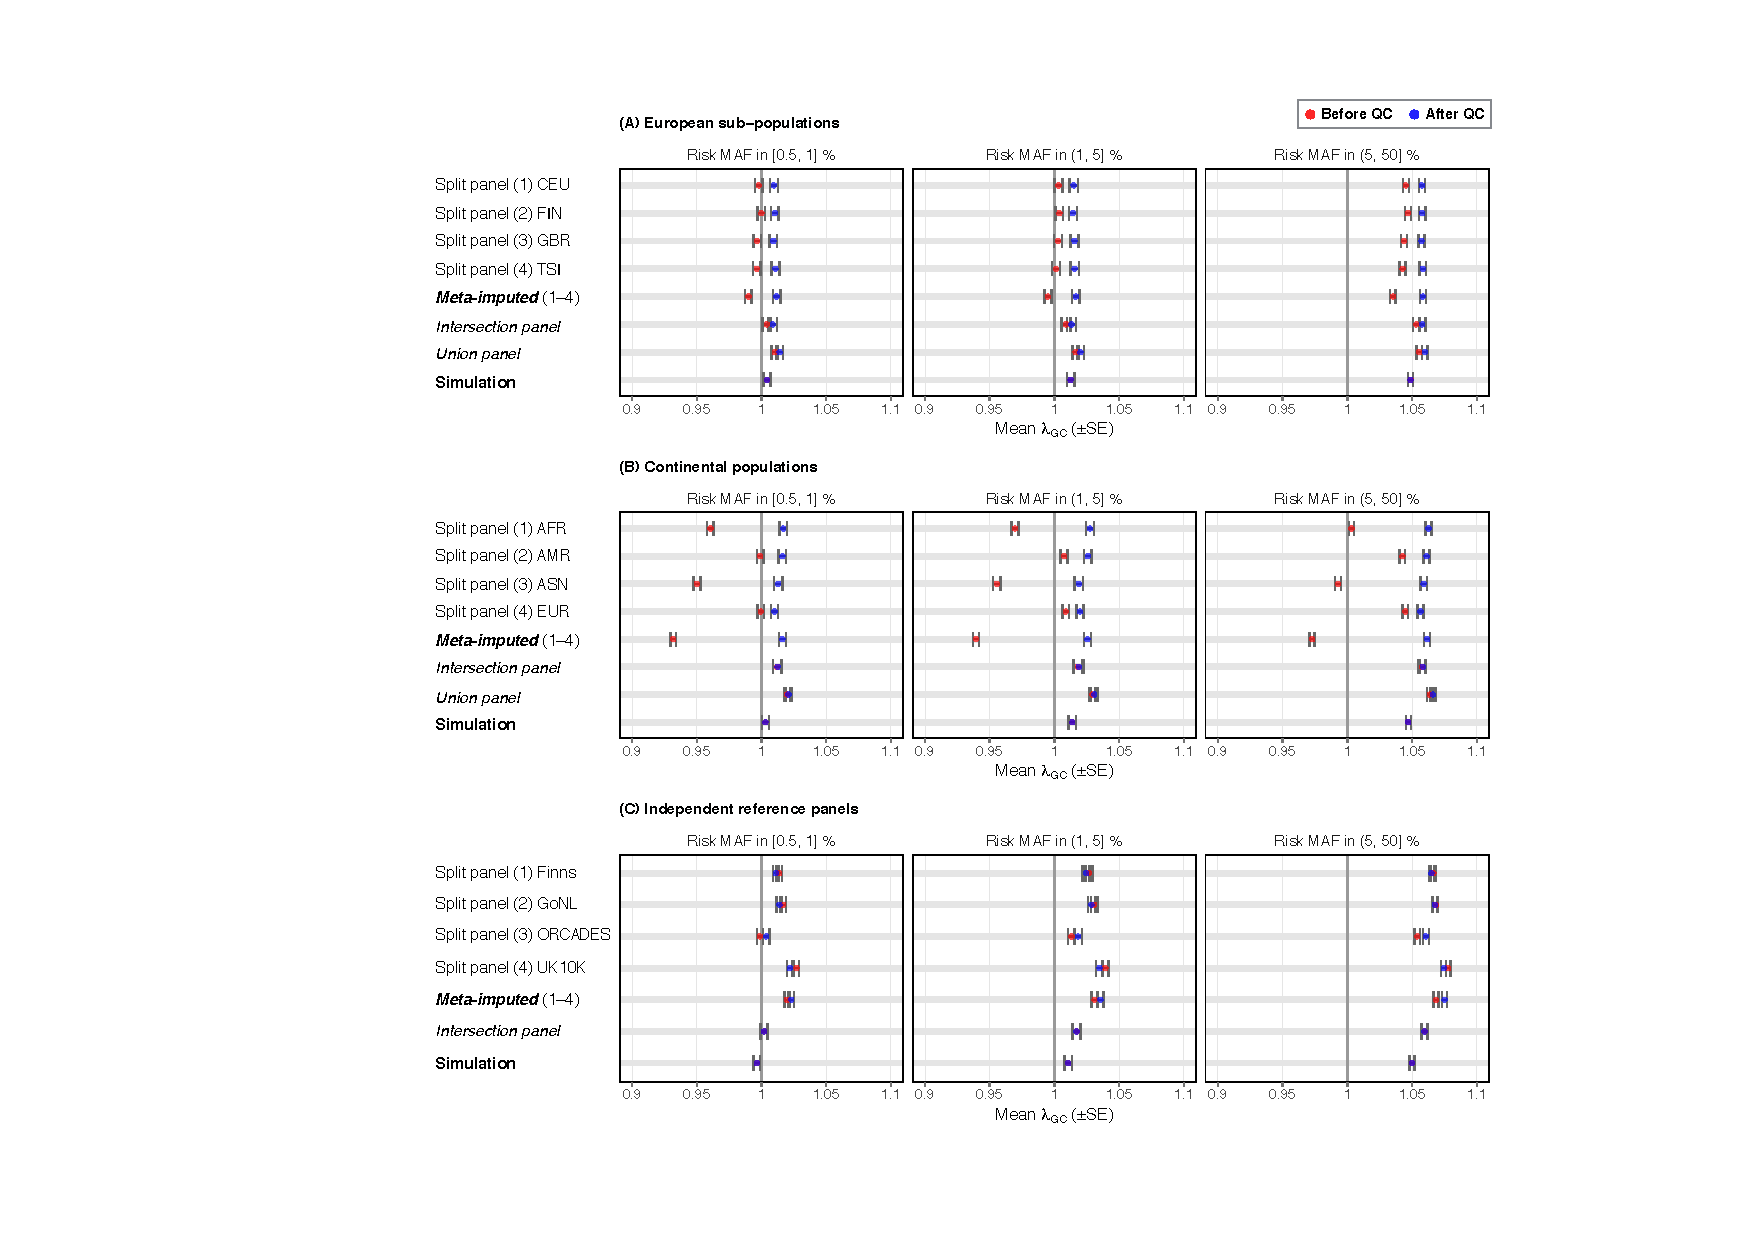
\includegraphics[width=\textwidth]{./img/ch2/association_lambda}
\Caption{Inflation observed in simulated case-control experiments}
{Genomic control inflation factor calculated before (\emph{red}) and after (\emph{blue}) variants were filtered in \gls{qc}, reported as mean $\lambda_\text{GC}$ over replicate association results by \gls{maf} of the simulated risk variants.}
{fig:power_lgc}
\end{figure}

%

Association results were inspected with regard to inflation before and after \gls{qc}; the difference is shown in \cpref{fig:power_lgc} where $\lambda_\text{GC}$ is shown as the average per \gls{maf} interval.
Inflation was slightly increased at higher frequencies; for example, association results using the non-imputed simulation dataset were at ${\lambda_\text{GC} \approx 1}$ on average in each scenario when the simulated risk variant was very low in frequency (${\text{MAF} \in [0.5, 1]\,\%}$), but increased to ${\lambda_\text{GC} \approx 1.05}$ for risk variants at higher frequencies (${\text{MAF} \in [5, 50]\,\%}$).
The impact of \gls{qc} was largest in Scenario~B, where association results of split panel imputed data were deflated (${\lambda_\text{GC} < 1}$) when seen in comparison to the simulated dataset or the intersection and union panels.
Notably, inflation was lowest for association results obtained from meta-imputed data in Scenarios~A and B.
The difference between $\lambda_\text{GC}$ calculated before and after \gls{qc} was negligible in Scenario~C.

%
%!TEX root = ../../main.tex


\begin{figure}[tb]
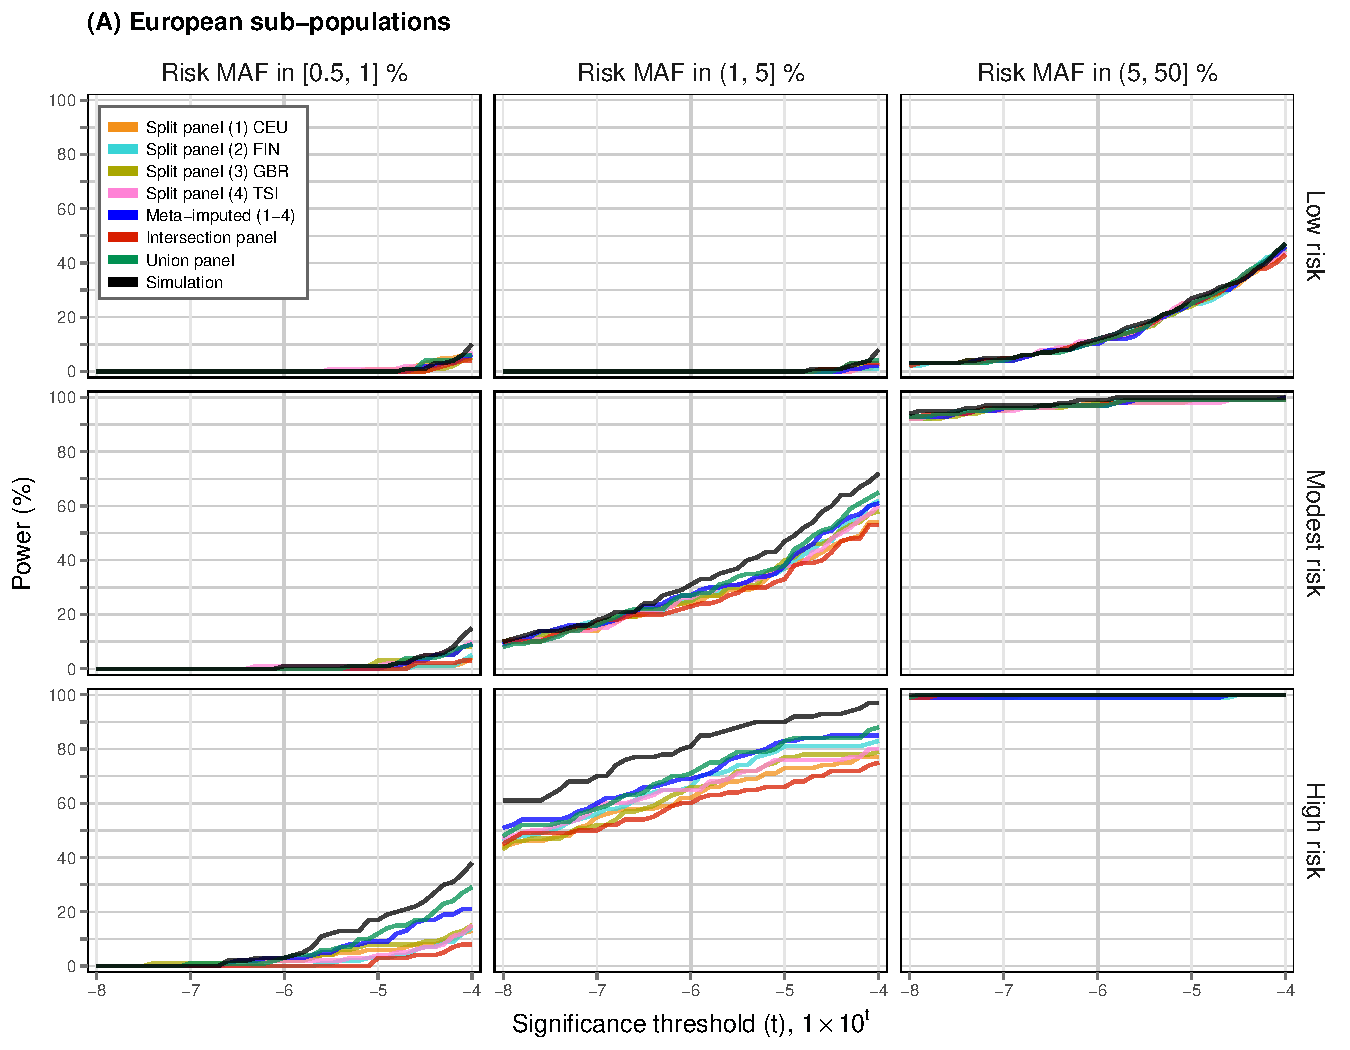
\includegraphics[width=\textwidth]{./img/ch2/plot_association_power_A}
\Caption{Power measured under a moving significance threshold}
{Power was calculated as the proportion of replicate association analyses ($n=100$, per combination of risk category and \gls{maf} interval) in which any signal reached significance within 1~\gls{Mb} around the position of a simulated risk variant.
A moving significance threshold between ${\pvalue\leq\num{1e-8}}$ and ${\pvalue\leq\num{1e-4}}$ was applied to each association dataset.\CorrectLabel}
{fig:gwas_power_A}
\end{figure}



\begin{figure}[tb]
\ContinuedFloat
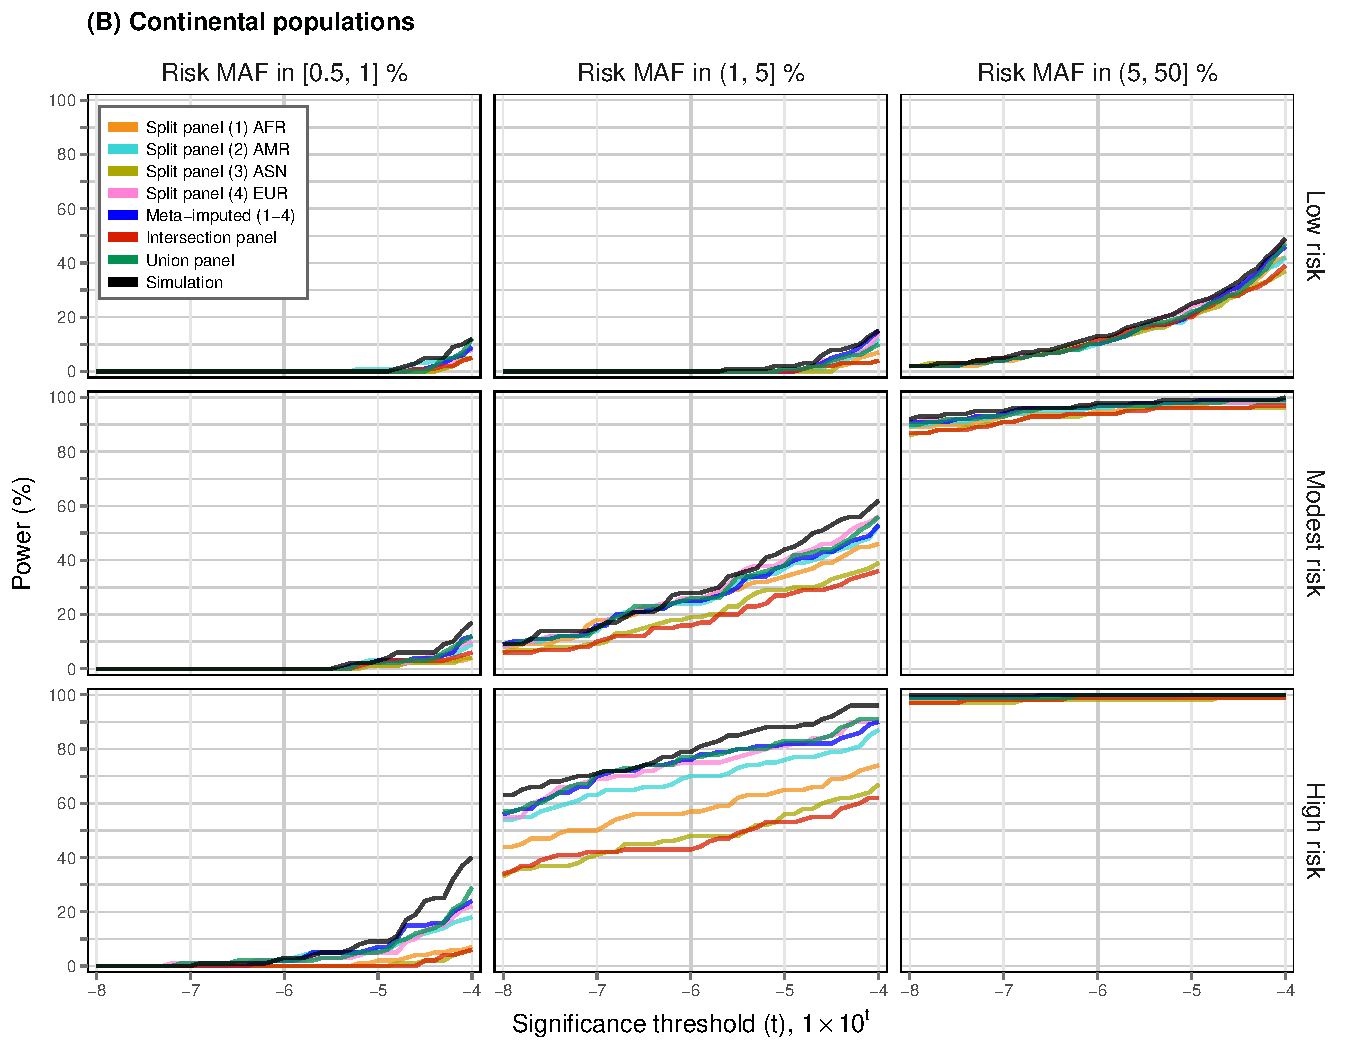
\includegraphics[width=\textwidth]{./img/ch2/plot_association_power_B}
\caption[]{Continued.\CorrectLabel}
\label{fig:gwas_power_B}
\end{figure}



\begin{figure}[tb]
\ContinuedFloat
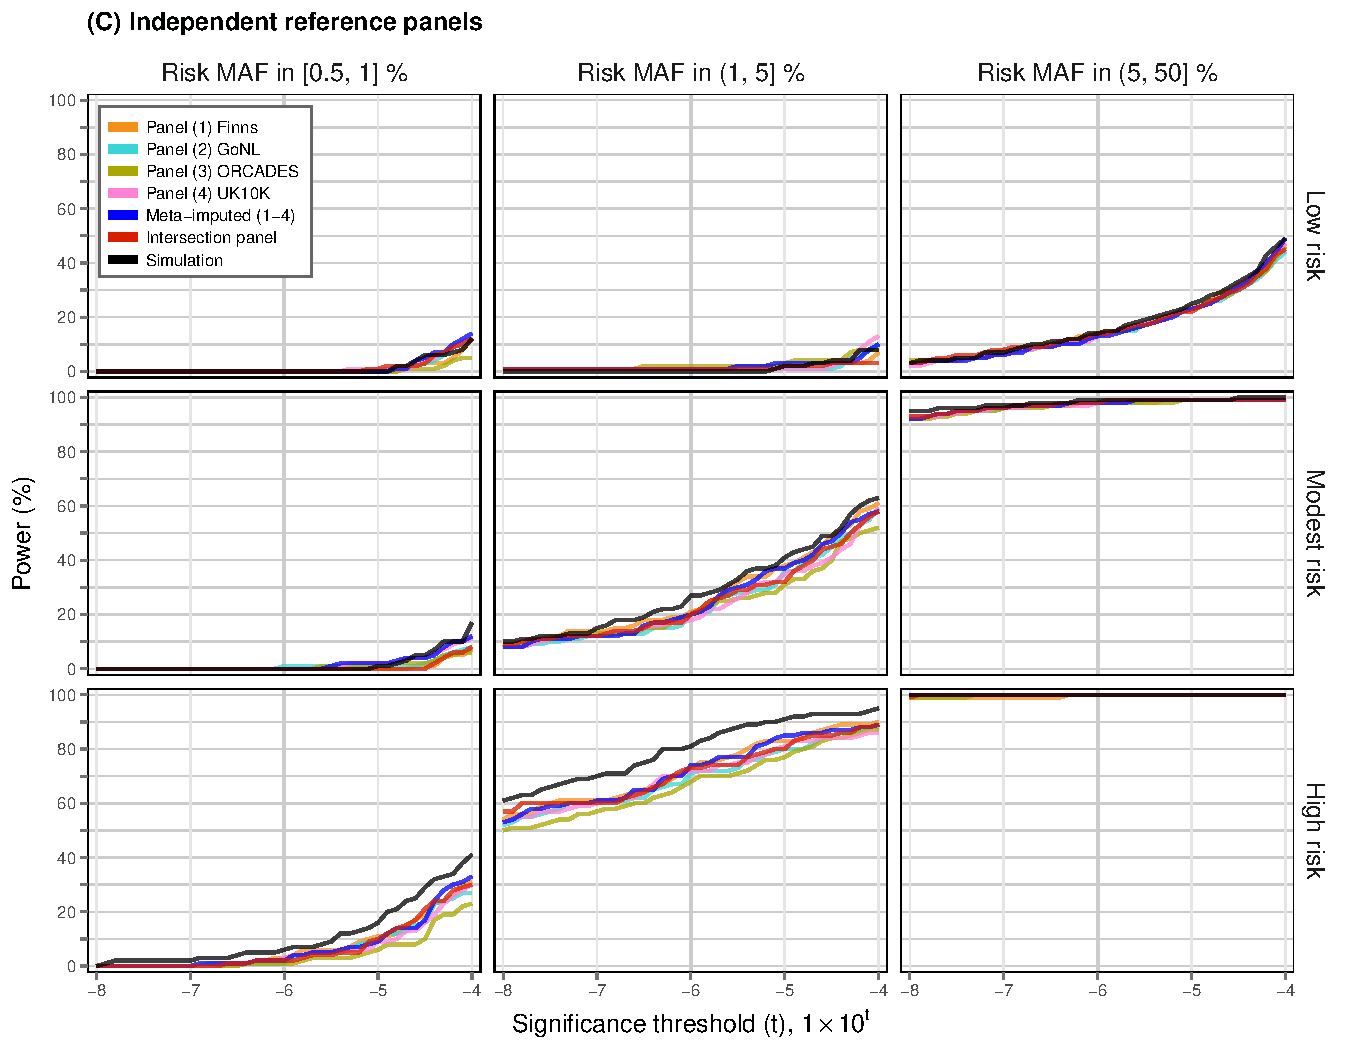
\includegraphics[width=\textwidth]{./img/ch2/plot_association_power_C}
\caption[]{Continued.\CorrectLabel}
\label{fig:gwas_power_C}
\end{figure}

%

%
% !TEX root = ../../main.tex


\begin{table}[!htb]
\Caption{Estimated power per imputation strategy}
{Power was estimated as the proportion of significant association signals found among replicate simulation experiments, for which \n{1} variant per simulation was selected at random from \n{3} \gls{maf} intervals (as specified in the table).
Each of the selected variants was simulated to act as a causal risk factor, where relative risk was simulated in \n{3} categories; low (${RR_{het}=1.2}$), modest (${RR_{het}=1.6}$), and high risk (${RR_{het}=2.0}$).
Power at a nominal significance threshold (${\pvalue\leq1\times10^{-6}}$) is reported at each combination of \gls{maf} interval and risk category.
The average difference ($\Delta_P$) in relation to the non-imputed simulation benchmark is given per \gls{maf} interval for each imputation strategy; the lowest average difference is highlighted (\textbf{bold}).
This table shows the results obtained for imputed and meta-imputed data in Scenario~A; results for Scenario~B (\pref{tab:stats_power_B}) and Scenario~C (\pref{tab:stats_power_C}) are shown separately.}
{tab:stats_power_A}
\centering
\TableUnits
\begin{threeparttable}
\begin{tabular}{%
 ll%
 S[table-format=5.0]%
 S[table-format=5.0]%
 S[table-format=5.0]%
 S[table-format=2.3]@{}S[table-format=1.3]%
 }
\multicolumn{7}{@{}l}{\bfseries (A) European sub-populations} \\
\toprule
 {Risk MAF (\%)} & {Panel} &
 \multicolumn{3}{c}{Power (\%), $\text{\pvalue} \leq 1\times10^{-6}$} &
 \multicolumn{2}{c}{$\Delta_P$ (\%)$^\ast$} \\
 \cmidrule(lr){3-5}
 \cmidrule(lr){6-7}
 & & {Low} & {Modest} & {High} & {Mean} & {($\pm$~SE)} \\
\otoprule
$[0.5, 1]$
 &  Split panel (1) CEU         &   0 &   0 &   2 &  2.53658  &  (0.48656) \\
 &  Split panel (2) FIN         &   0 &   0 &   0 &  3.04065  &  (0.51969) \\
 &  Split panel (3) GBR         &   0 &   0 &   2 &  2.09756  &  (0.44389) \\
 &  Split panel (4) TSI         &   0 &   1 &   2 &  2.30894  &  (0.50863) \\
\cmidrule(lr){3-7}
 &  Meta-imputed (1-4)          &   0 &   0 &   3 &  1.55284  &  (0.28912) \\
 & \slshape  Intersection panel &   0 &   0 &   0 &  3.36585  &  (0.59253) \\
 & \slshape  Union panel        &   0 &   0 &   3 & \bfseries 1.04878  &  (0.20614) \\
\cmidrule(lr){2-7}
$(1, 5]$
 &  Split panel (1) CEU         &   0 &  24 &  62 &  8.56097  &  (0.72925) \\
 &  Split panel (2) FIN         &   0 &  25 &  66 &  6.37398  &  (0.54277) \\
 &  Split panel (3) GBR         &   0 &  25 &  66 &  7.43089  &  (0.67039) \\
 &  Split panel (4) TSI         &   0 &  26 &  65 &  7.12195  &  (0.60514) \\
\cmidrule(lr){3-7}
 &  Meta-imputed (1-4)          &   0 &  27 &  69 &  4.95934  &  (0.43109) \\
 & \slshape  Intersection panel &   0 &  23 &  60 &  9.56097  &  (0.84577) \\
 & \slshape  Union panel        &   0 &  27 &  71 & \bfseries 4.84552  &  (0.41641) \\
\cmidrule(lr){2-7}
$(5, 50]$
 &  Split panel (1) CEU         &  11 &  98 & 100 &  0.78048  &  (0.06784) \\
 &  Split panel (2) FIN         &  12 &  98 &  99 &  0.89430  &  (0.07004) \\
 &  Split panel (3) GBR         &  11 &  98 & 100 &  0.82113  &  (0.08327) \\
 &  Split panel (4) TSI         &  11 &  97 & 100 &  0.74796  &  (0.08986) \\
\cmidrule(lr){3-7}
 &  Meta-imputed (1-4)          &  10 &  97 &  99 &  0.95934  &  (0.06868) \\
 & \slshape  Intersection panel &  11 &  97 & 100 &  0.63414  &  (0.07325) \\
 & \slshape  Union panel        &  11 &  97 & 100 & \bfseries 0.53658  &  (0.06760) \\
 \bottomrule
\end{tabular}
\begin{tablenotes}\footnotesize\DefaultUnits
 \item[{${\ast}$}] Average difference in power between simulated and (meta-)imputed association results ($\Delta_P$);
 averaged over risk category (low, modest, and high risk) and association signals detected at a moving significance threshold; between ${\pvalue\leq\num{1e-08}}$ and ${\pvalue\leq\num{1e-04}}$.
\end{tablenotes}
\end{threeparttable}
\end{table}



\begin{table}[!htb]
\ContinuedFloat
\small
\caption[]{Continued.}
\label{tab:stats_power_B}
\centering
\TableUnits
\begin{threeparttable}
\begin{tabular}{%
	ll%
	S[table-format=5.0]%
	S[table-format=5.0]%
	S[table-format=5.0]%
	S[table-format=2.3]@{}S[table-format=1.3]%
	}
 \multicolumn{7}{@{}l}{\bfseries (B) Continental populations} \\
\toprule
 {Risk MAF (\%)} & {Panel} &
 \multicolumn{3}{c}{Power (\%), $\text{\pvalue} \leq 1\times10^{-6}$} &
 \multicolumn{2}{c}{$\Delta_P$ (\%)$^\ast$} \\
 \cmidrule(lr){3-5}
 \cmidrule(lr){6-7}
 & & {Low} & {Modest} & {High} & {Mean} & {($\pm$~SE)} \\
\otoprule
$[0.5, 1]$
 &  Split panel (1) AFR        &   0 &   0 &   0 &  3.00000  &  (0.54124)  \\
 &  Split panel (2) AMR        &   0 &   0 &   3 &  1.48780  &  (0.33724)  \\
 &  Split panel (3) ASN        &   0 &   0 &   0 &  3.20325  &  (0.58263)  \\
 &  Split panel (4) EUR        &   0 &   0 &   2 &  1.55284  &  (0.29640)  \\
\cmidrule(lr){3-7}
 &  Meta-imputed (1-4)         &   0 &   0 &   2 & \bfseries 1.22764  &  (0.24728)  \\
 & \slshape Intersection panel &   0 &   0 &   0 &  3.04878  &  (0.57894)  \\
 & \slshape Union panel        &   0 &   0 &   2 &  1.30081  &  (0.24731)  \\
\cmidrule(lr){2-7}
$(1, 5]$
 &  Split panel (1) AFR        &   0 &  25 &  57 &  9.36585  &  (0.86594)  \\
 &  Split panel (2) AMR        &   0 &  24 &  70 &  5.21951  &  (0.44225)  \\
 &  Split panel (3) ASN        &   0 &  19 &  48 & 14.61788  &  (1.19717)  \\
 &  Split panel (4) EUR        &   0 &  26 &  75 &  2.71544  &  (0.25931)  \\
\cmidrule(lr){3-7}
 &  Meta-imputed (1-4)         &   0 &  25 &  76 &  3.06504  &  (0.29517)  \\
 & \slshape Intersection panel &   0 &  16 &  43 & 15.54471  &  (1.24817)  \\
 & \slshape Union panel        &   0 &  26 &  77 & \bfseries 2.65040  &  (0.24760)  \\
\cmidrule(lr){2-7}
$(5, 50]$
 &  Split panel (1) AFR        &  11 &  95 &  99 &  1.98373  &  (0.10389)  \\
 &  Split panel (2) AMR        &  10 &  96 &  99 &  1.40650  &  (0.10942)  \\
 &  Split panel (3) ASN        &  12 &  94 &  98 &  2.82926  &  (0.17686)  \\
 &  Split panel (4) EUR        &  11 &  97 & 100 & \bfseries 0.65040  &  (0.07208)  \\
\cmidrule(lr){3-7}
 &  Meta-imputed (1-4)         &  10 &  97 & 100 &  0.95121  &  (0.08931)  \\
 & \slshape Intersection panel &  12 &  94 &  99 &  2.56097  &  (0.17322)  \\
 & \slshape Union panel        &  10 &  97 & 100 &  1.13821  &  (0.09259)  \\
\bottomrule
\end{tabular}
\begin{tablenotes}\footnotesize\DefaultUnits
 \item[{${\ast}$}] See \cref{tab:stats_power_A}{A} (\pref{tab:stats_power_A}).
\end{tablenotes}
\end{threeparttable}
\end{table}



\begin{table}[!htb]
\ContinuedFloat
\small
\caption[]{Continued.}
\label{tab:stats_power_C}
\centering
\TableUnits
\begin{threeparttable}
\begin{tabular}{%
	ll%
  S[table-format=5.0]%
	S[table-format=5.0]%
	S[table-format=5.0]%
  S[table-format=2.3]@{}S[table-format=1.3]%
	}
\multicolumn{7}{@{}l}{\bfseries (C) Independent reference panels} \\
\toprule
 {Risk MAF (\%)} & {Panel} &
 \multicolumn{3}{c}{Power (\%), $\text{\pvalue} \leq 1\times10^{-6}$} &
 \multicolumn{2}{c}{$\Delta_P$ (\%)$^\ast$} \\
 \cmidrule(lr){3-5}
 \cmidrule(lr){6-7}
 & & {Low} & {Modest} & {High} & {Mean} & {($\pm$~SE)} \\
\otoprule
$[0.5, 1]$
 &  Panel (1) Finns             &   0 &   0 &   3 &  1.91869  &  (0.24910)  \\
 &  Panel (2) GoNL              &   0 &   1 &   1 &  1.86178  &  (0.29007)  \\
 &  Panel (3) ORCADES           &   0 &   0 &   1 &  2.80487  &  (0.41571)  \\
 &  Panel (4) UK10K             &   0 &   0 &   3 &  1.68292  &  (0.30485)  \\
\cmidrule(lr){3-7}
 &  Meta-imputed (1-4)          &   0 &   0 &   2 & \bfseries 1.31707  &  (0.24796)  \\
 & \slshape Intersection panel  &   0 &   0 &   2 &  1.85365  &  (0.25806)  \\
\cmidrule(lr){2-7}
$(1, 5]$
 &  Panel (1) Finns             &   1 &  21 &  73 & \bfseries 3.11382  &  (0.34348)  \\
 &  Panel (2) GoNL              &   1 &  20 &  71 &  4.94308  &  (0.43645)  \\
 &  Panel (3) ORCADES           &   2 &  20 &  68 &  5.76422  &  (0.57214)  \\
 &  Panel (4) UK10K             &   1 &  18 &  72 &  4.78861  &  (0.42766)  \\
\cmidrule(lr){3-7}
 &  Meta-imputed (1-4)          &   1 &  20 &  74 &  3.51219  &  (0.35720)  \\
 & \slshape Intersection panel  &   1 &  20 &  73 &  4.19512  &  (0.38716)  \\
\cmidrule(lr){2-7}
$(5, 50]$
 &  Panel (1) Finns             &  14 &  98 & 100 &  0.68292  &  (0.06663)  \\
 &  Panel (2) GoNL              &  13 &  98 & 100 &  0.82113  &  (0.10263)  \\
 &  Panel (3) ORCADES           &  14 &  98 & 100 &  0.91056  &  (0.09590)  \\
 &  Panel (4) UK10K             &  13 &  98 & 100 &  0.78048  &  (0.07875)  \\
\cmidrule(lr){3-7}
 &  Meta-imputed (1-4)          &  13 &  98 & 100 &  0.74796  &  (0.07880)  \\
 & \slshape Intersection panel  &  14 &  98 & 100 & \bfseries 0.54471  &  (0.09181)  \\
\bottomrule
\end{tabular}
\begin{tablenotes}\footnotesize\DefaultUnits
 \item[{${\ast}$}] See \cref{tab:stats_power_A}{A} (\pref{tab:stats_power_A}).
\end{tablenotes}
\end{threeparttable}
\end{table}

%

Association results for each imputation strategy (referring to results obtained on genotype data imputed from available reference panels and meta-imputation) were separately evaluated with regard to each combination of risk category and the \gls{maf} interval from which simulated risk variants were selected.
The distribution of power measured under a moving significance threshold (between ${\pvalue\leq1\times10^{-8}}$ and ${\pvalue\leq1\times10^{-4}}$) is shown in \cref{fig:gwas_power_A}; for Scenario~A (\pref{fig:gwas_power_A}), B~(\pref{fig:gwas_power_B}), and~C~(\pref{fig:gwas_power_C}).
The results are summarised in \cref{tab:stats_power_A}, for power measured at the nominal significance threshold (${\pvalue\leq1\times10^{-6}}$) and the average difference to the non-imputed simulation benchmark ($\Delta_P$) along the moving threshold, averaged per \gls{maf} interval of simulated risk variants; for Scenario~A (\pref{tab:stats_power_A}), B~(\pref{tab:stats_power_B}), and~C~(\pref{tab:stats_power_C}).

The union panel was seen with the lowest average difference in power at very low frequencies of the simulated risk variant (${\text{MAF} \in [0.5, 1]\,\%}$) in Scenario~A, where $\Delta_P$ was \MeanValue{1.04878}{0.20614}.
Meta-imputation showed the lowest average difference at very low \gls{maf} in Scenario~B, $\Delta_P=\MeanPercent{1.22764}{0.24728}$, as well as Scenario~C, $\Delta_P=\MeanPercent{1.31707}{0.24796}$; but recall that Scenario~C (independent reference panels) did not contain a union panel.
However, even in the high risk category in each scenario, estimated power did not exceed 3\% for any imputation strategy when the simulated risk variant was very low in frequency, such that observed differences were negligible as these could be attributed to stochastic noise.
Similarly, observed differences were small in each risk category when causal variants were selected from the high frequency interval (${\text{MAF} \in [5,50]\,\%}$), where the lowest average difference in power was recorded for the union panel in Scenario~A, $\Delta_P=\MeanPercent{0.53658}{0.06760}$, the EUR split panel in B, \MeanPercent{0.65040}{0.07208}, and the intersection panel in C, \MeanPercent{0.54471}{0.09181}.
However, note that ${\Delta_P<1\%}$ in each strategy at high risk \gls{maf} in Scenarios~A and C, but where some of the strategies showed larger differences in Scenario~B, \eg the ASN split panel and the intersection panel; \MeanPercent{2.82926}{0.17686} and \MeanPercent{2.56097}{0.17322}, respectively.

Noticeable differences were seen among imputation strategies for simulated risk variants selected at low frequency (${\text{MAF} \in [1, 5]\,\%}$).
The union panel was recorded with the lowest difference in power relative to the non-imputed simulation benchmark in Scenarios~A and B, \MeanPercent{4.84552}{0.41641} and \MeanPercent{2.65040}{0.24760}, respectively, whereas the intersection panel had the highest difference, \MeanPercent{9.56097}{0.84577} and \MeanPercent{15.54471}{1.24817}, respectively.
Notably, meta-imputation was similarly close as the union panel and outperformed the other imputation strategies in Scenario~A, \MeanPercent{4.95934}{0.43109}.
For example, at a nominal threshold (${\pvalue\leq1\times10^{-6}}$), the union panel reached 71\% power and meta-imputation 69\% in the high risk category.
In Scenario~B, the power observed for meta-imputed data was high by comparison,
\eg 76\% power at high risk, compared to 77\% for the union panel and 43\% for the intersection panel; however, $\Delta_P$ measured for meta-imputation was \MeanPercent{3.06504}{0.29517}, which was lower in the EUR split panel, \MeanPercent{2.71544}{0.25931}, reaching 76\% in the high risk category.
In Scenario~C, the \emph{Finns} panel showed the lowest difference in power, \MeanPercent{3.11382}{0.34348}, and the \emph{ORCADES} panel the highest, \MeanPercent{5.76422}{0.57214}; yet, meta-imputation ranked \nth{2} best among the strategies compared, \MeanPercent{3.51219}{0.35720}, but \nth{1} in the high risk category with 74\% power (compared to 73\% and 68\% for \emph{Finns} and \emph{ORCADES}, respectively).



%
\section{Discussion}
\label{metaimpute_discussion}
%

Meta-imputation was presented as a novel approach to integrate reference data after imputation into a common study sample, but the idea of combining genotype data imputed from different reference panels has been investigated before.
\Citet{Chen:2013jx} used low to high-depth sequencing data as references for imputations into a given study sample, where imputed data have been matched and combined at overlapping sites, but such that variant genotypes imputed from the high-quality panel were included preferentially.
They have shown that this approach improved overall accuracy compared to each separately imputed dataset.
Here, I considered several variations of this approach which I evaluated using several reference datasets as available in different use case scenarios.
Notably, the meta-imputation method does not require prior knowledge to guide the merging process (such as high or low quality of each dataset considered), which instead is determined by summary information derived directly from imputed genotype data.

The results I presented in this chapter showed that the combination of genotype data may indeed result in an increase of accuracy across the allele frequency spectrum, but where the largest improvements were seen for low-frequency variants (\eg 1--5\% \gls{maf}).
I showed that meta-imputation improved genotype accuracy such that single-reference imputations were outperformed (\eg in Scenario~A), but also that meta-imputed genotype data may not further increase accuracy if a reference is highly accurate by itself (\eg the EUR sample in Scenario~B).
Nonetheless, the inclusion of other, more distantly related reference haplotypes may not affect the accuracy of the resulting meta-imputed dataset (\eg the AFR or ASN samples for imputation into the European sample in Scenario~B).

Meta-imputed genotype data were contrasted with data obtained in imputations from corresponding, larger datasets, which contained the unified sample across the datasets considered in meta-imputation; \ie the intersection and the union of variants present across the other reference datasets, respectively.
Although meta-imputation did not perform markedly better in terms of accuracy (measured at the same variant sites), I showed that meta-imputation generally outperformed the intersection panel, in terms of power to detect significant association signals, due to the low coverage retained at the intersection of variants across available reference data.
However, note that meta-imputation combined data such that the resulting coverage was identical to the coverage of the union panel; meta-imputed data was overall similar to using the union reference for imputation, with regard to both accuracy and power.

In conclusion, these results suggest that meta-imputation is a viable approach to combine genotype data such that a larger, unified dataset of imputed genotypes is available for association analysis.
However, it is unlikely to increase accuracy and power further than possible with imputation from a large, canonical reference; \eg the reference dataset provided by the \acrfull{hrc}.
Yet, future \gls{gwa} studies may benefit from meta-imputation, for example, in situations when researchers have to choose from a collection of available reference datasets, or to increase the coverage of imputed data in general.
The meta-imputation algorithm, as presented in this chapter, is available as a computational tool which I implemented in \cpp.\footnote{Meta-imputation software (\texttt{meta-impute}): \url{https://github.com/pkalbers/meta-impute}}
